%!Mode:: "TeX:UTF-8"
\documentclass{beamer}
\usepackage{xeCJK}
\usepackage{xcolor}
\usepackage{listings}
\usepackage{soul}
\usepackage{ulem}
\usepackage{url}
\usepackage{graphicx}
\usepackage{multirow}
\usepackage{hepunits}

%\setCJKmainfont{AR PL SungtiL GB}
%\setCJKmonofont{AR PL SungtiL GB}
\setCJKmainfont{SimSun}
\setCJKmonofont{SimSun}

\definecolor{dkgreen}{rgb}{0,0.6,0}
\definecolor{gray}{rgb}{0.5,0.5,0.5}
\definecolor{mauve}{rgb}{0.58,0,0.82}

\lstset{
    language=sh,
    %basicstyle=\footnotesize\ttfamily,
    basicstyle=\scriptsize\ttfamily,
    frameround=tttt,
    frame=single,
    keywordstyle=\color{blue},
    commentstyle=\color{dkgreen},
    stringstyle=\color{mauve},
    numbers=left,
    numberstyle=\tiny\color{gray},
    numbersep=5pt,
    escapeinside={(*@}{@*)},
    %otherkeywords={$, \{, \}, \[, \]},
}

%\setbeamertemplate{footline}[frame number]
\setbeamertemplate{navigation symbols}{}
\usetheme{Madrid}
\begin{document}

\title{2013年04月份考核报告}
\author{
    \texorpdfstring{林韬
                    \newline
                    \href{mailto:lintao@ihep.ac.cn}
                    {\footnotesize\ttfamily{lintao@ihep.ac.cn}}}
                    {Lin Tao}
}
\institute{IHEP}

\maketitle

\begin{frame}
    \frametitle{OUTLINE}
    \tableofcontents
\end{frame}

\section{江门中微子实验探测器模拟及离线软件}
    
\begin{frame}
    \begin{center}
        \LARGE 江门中微子实验探测器模拟及离线软件
    \end{center}
\end{frame}

\begin{frame}
    \frametitle{江门中微子实验软件工作}
    \begin{itemize}
        \item 离线软件环境的维护。
        \item 探测器模拟软件的开发。
        \item 几种不同方案探测器的模拟。
            \begin{itemize}
                \item 能量分辨率的研究,
                \item 放射性本底对能量分辨率的影响。
            \end{itemize}
        \item 基于Sniper离线框架的探测器模拟软件。
    \end{itemize}
\end{frame}

\subsection{离线软件环境的维护}

\begin{frame}
    \frametitle{离线软件环境的维护}
    \begin{itemize}
        \item 外部库的重新安装(由于panfs盘的下线)。
            \begin{itemize}
                \item 目前迁移至{\tt
                    /afs/ihep.ac.cn/soft/dayabay/jmne/external/local}
                \item 图形库Qt的安装。目前编译的Geant4使用Qt作为UI。
            \end{itemize}
        \item 完善了geant4中使用的数据集(
              原先的geant4没有安装完整的数据集,导致看不到放射性衰变)。
        \item 由于离线软件将使用subversion进行版本控制,
              因此配置了svn服务器。并使用Trac对svn进行用户授权。
        \item 原先的探测器模拟程序目前仍旧使用git进行版本控制。
    \end{itemize}
\end{frame}

\begin{frame}
    \frametitle{使用Trac对svn进行用户及权限管理}
    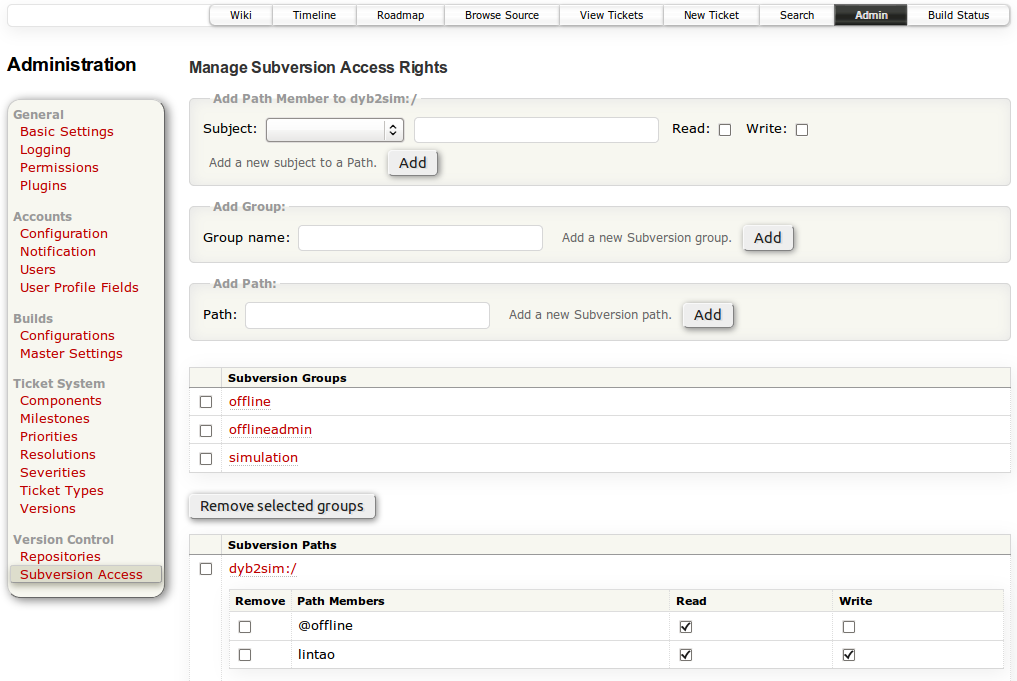
\includegraphics[width=12cm,keepaspectratio]{data/trac_svn.png}
\end{frame}

\subsection{模拟软件的开发}

\begin{frame}
    \frametitle{模拟软件的开发}
    \begin{itemize}
        \item 产生子
            \begin{itemize}
                \item 支持按照时间将HepEvt事例拆分成子事例
                \item 支持GENIE中产生的RooTracker格式(加速器中微子)
            \end{itemize}
        \item 物理过程
            \begin{itemize}
                \item 修正了Optical Rayleigh Scattering的bug。
                      (由于大亚湾一期的Rayleigh Scattering是基于Geant4 9.2,
                       而到9.4中这个bug才修复。)
                       \footnote{由北大王思广指出}
                \item 添加了中子俘获散射截面及末态信息数据。
                      (一期中使用了NNDC核数据库的数据,
                      而在我们初期的模拟中,我们没有注意到要使用这些数据。)
                       \footnote{由山大陈泉佑指出}
                \item 对旧式的低能电磁过程及新式的Livermore模型进行比较。
            \end{itemize}
        \item PMT相关的研究
            \begin{itemize}
                \item 对PMT几何进行了研究。初步了解TorusStack的构建方法。
                \item 修正20英寸Torus Stack的问题。
                      \footnote{由武大丁雪峰指出}
                \item 尝试对PMT的构造进行改造(未完成,仍有overlap的问题)。
            \end{itemize}
    \end{itemize}
\end{frame}

\begin{frame}
    \frametitle{不同构造方式的PMT}
    \begin{columns}
        \column{6.0cm}
        \begin{figure}
            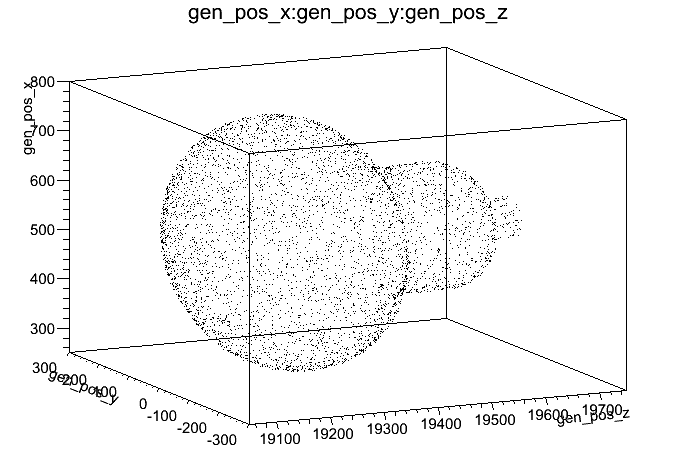
\includegraphics[width=6cm,keepaspectratio]{data/torusstack_PMT.png}
            \caption{Torus Stack方式构建}
        \end{figure}
        \column{6.0cm}
        \begin{figure}
            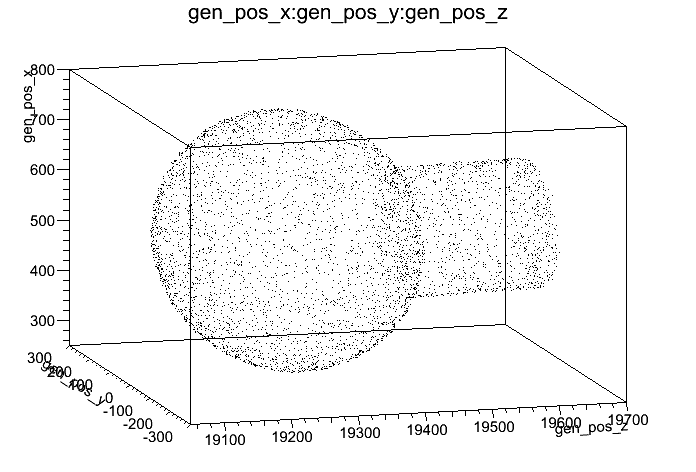
\includegraphics[width=6cm,keepaspectratio]{data/ellipsoid_PMT.png}
            \caption{Ellipsoid方式构建}
        \end{figure}
    \end{columns}
\end{frame}

\subsection{不同方案探测器的模拟}

\begin{frame}
    \frametitle{不同方案探测器的模拟}
    \begin{itemize}
        \item 主要研究探测器的能量分辨率及本底对能量分辨率的影响。
            \begin{itemize}
                \item 纯钢罐方案
                \item 液闪+有机玻璃+水屏蔽(PMT泡在水中)
                \item 液闪+有机玻璃罐
                \item 液闪+有机玻璃罩
                \item 1mm液闪对本底的影响
            \end{itemize}
    \end{itemize}
\end{frame}

\begin{frame}
    \frametitle{纯钢罐: 2*0.511MeV}

\begin{tabular}{|c|cc|cc|cc|}
\hline
% line one
 & \multicolumn{2}{|c|}{No Smear} 
 & \multicolumn{2}{|c|}{Smear 5cm}
 & \multicolumn{2}{|c|}{Smear 10cm}
\\
\hline
% line two
 & mean & sigma
 & mean & sigma
 & mean & sigma
\\
\hline
% line 4
0.5MHz,200ns
 & 0.9907 & 0.02983 
 & 0.9932 & 0.02997
 & 0.9929 & 0.03015
\\
\hline
% line 5
0.5MHz,300ns
 & 0.9849 & 0.03012
 & 0.9888 & 0.02999
 & 0.9868 & 0.03039
\\
\hline
% line 6
0.5MHz,400ns
& \multirow{2}{*}{0.9812} & \multirow{2}{*}{0.03059}
& \multirow{2}{*}{0.9825} & \multirow{2}{*}{0.03028}
& \multirow{2}{*}{0.9807} & \multirow{2}{*}{0.03047}
\\
\cline{1-1}
1.0MHz,200ns
 &  & 
 &  & 
 &  & 
\\
\hline
% line 7
0.5MHz,500ns
 & 0.9748 & 0.03104
 & 0.9741 & 0.03174
 & 0.9726 & 0.03205
\\
\hline
% line 5
1.0MHz,300ns
& \multirow{2}{*}{0.9646} & \multirow{2}{*}{0.03194}
& \multirow{2}{*}{0.9668} & \multirow{2}{*}{0.03281}
& \multirow{2}{*}{0.964} & \multirow{2}{*}{0.03292}
\\
\cline{1-1}
1.5MHz,200ns
 &  & 
 &  & 
 &  & 
\\
\hline
% line 6
1.0MHz,400ns
 & 0.9513  & 0.03328
 & 0.9507  & 0.03254
 & 0.9526  & 0.03396
\\
\hline
% line 7
1.0MHz,500ns
 & 0.9406 & 0.03513
 & 0.9413 & 0.03563
 & 0.9392 & 0.03494
\\
\hline
% line 6
1.5MHz,400ns
 & 0.9286 & 0.03801
 & 0.9320 & 0.03988
 & 0.9304 & 0.03934
\\
\hline
% line 7
1.5MHz,500ns
 & 0.9125  & 0.04266
 & 0.9119  & 0.04241
 & 0.9155  & 0.04451
\\
\hline
\end{tabular}

\end{frame}

\begin{frame}
    \frametitle{纯钢罐: 2.22MeV}

\begin{tabular}{|c|cc|cc|cc|}
\hline
% line one
 & \multicolumn{2}{|c|}{No Smear} 
 & \multicolumn{2}{|c|}{Smear 5cm}
 & \multicolumn{2}{|c|}{Smear 10cm}
\\
\hline
% line two
 & mean & sigma
 & mean & sigma
 & mean & sigma
\\
\hline
% line 4
0.5MHz,200ns
 & 0.9973  & 0.02364
 & 0.9975  & 0.02378
 & 0.9972  & 0.02414
\\
\hline
% line 5
0.5MHz,300ns
 & 0.9948  & 0.02369
 & 0.9940  & 0.02377
 & 0.9942  & 0.02414
\\
\hline
% line 6
0.5MHz,400ns
& \multirow{2}{*}{0.9916} & \multirow{2}{*}{0.02386}
& \multirow{2}{*}{0.9910} & \multirow{2}{*}{0.02403}
& \multirow{2}{*}{0.9918} & \multirow{2}{*}{0.02434}
\\
\cline{1-1}
1.0MHz,200ns
 &  & 
 &  & 
 &  & 
\\
\hline
% line 7
0.5MHz,500ns
 & 0.9880 &  0.02406
 & 0.9882 &  0.02418
 & 0.9880 &  0.02447
\\
\hline
% line 5
1.0MHz,300ns
& \multirow{2}{*}{0.9834} & \multirow{2}{*}{0.02424}
& \multirow{2}{*}{0.9829} & \multirow{2}{*}{0.02456}
& \multirow{2}{*}{0.9829} & \multirow{2}{*}{0.02497}
\\
\cline{1-1}
1.5MHz,200ns
 &  & 
 &  & 
 &  & 
\\
\hline
% line 6
1.0MHz,400ns
 & 0.9766 &  0.02553
 & 0.9774 &  0.02593
 & 0.9771 &  0.02607
\\
\hline
% line 7
1.0MHz,500ns
 & 0.9708 &  0.027
 & 0.9710 &  0.02687
 & 0.9718 &  0.02695
\\
\hline
% line 6
1.5MHz,400ns
 & 0.9646 &  0.02897
 & 0.9653 &  0.02935
 & 0.9654 &  0.02938
\\
\hline
% line 7
1.5MHz,500ns
 & 0.9554 &  0.03141
 & 0.9552 &  0.03159
 & 0.9556 &  0.03217
\\
\hline
\end{tabular}

\end{frame}

\begin{frame}
    \frametitle{纯钢罐: 1.173MeV+1.333MeV}

\begin{tabular}{|c|cc|cc|cc|}
\hline
% line one
 & \multicolumn{2}{|c|}{No Smear} 
 & \multicolumn{2}{|c|}{Smear 5cm}
 & \multicolumn{2}{|c|}{Smear 10cm}
\\
\hline
% line two
 & mean & sigma
 & mean & sigma
 & mean & sigma
\\
\hline
% line 4
0.5MHz,200ns
 & 0.9982 &  0.02131
 & 0.9980 &  0.02144
 & 0.9981 &  0.02178
\\
\hline
% line 5
0.5MHz,300ns
 & 0.9952 &  0.02132
 & 0.9962 &  0.02418
 & 0.9957 &  0.0218
\\
\hline
% line 6
0.5MHz,400ns
& \multirow{2}{*}{0.9918} & \multirow{2}{*}{0.02139}
& \multirow{2}{*}{0.9916} & \multirow{2}{*}{0.02146}
& \multirow{2}{*}{0.9922} & \multirow{2}{*}{0.02184}
\\
\cline{1-1}
1.0MHz,200ns
 &  & 
 &  & 
 &  & 
\\
\hline
% line 7
0.5MHz,500ns
 & 0.9875 &  0.02152
 & 0.9817 &  0.02173
 & 0.9817 &  0.0222
\\
\hline
% line 5
1.0MHz,300ns
& \multirow{2}{*}{0.9864} & \multirow{2}{*}{0.02192}
& \multirow{2}{*}{0.9861} & \multirow{2}{*}{0.02213}
& \multirow{2}{*}{0.9860} & \multirow{2}{*}{0.02218}
\\
\cline{1-1}
1.5MHz,200ns
 &  & 
 &  & 
 &  & 
\\
\hline
% line 6
1.0MHz,400ns
 & 0.9776 &  0.02323
 & 0.9782 &  0.02323
 & 0.9784 &  0.02298
\\
\hline
% line 7
1.0MHz,500ns
 & 0.9749 &  0.02372
 & 0.9748 &  0.02379
 & 0.9752 &  0.02442
\\
\hline
% line 6
1.5MHz,400ns
 & 0.9658 &  0.02599
 & 0.9658 &  0.02636
 & 0.9661 &  0.02667
\\
\hline
% line 7
1.5MHz,500ns
 & 0.9578 &  0.02874
 & 0.9576 &  0.02932
 & 0.9580 &  0.02975
\\
\hline
\end{tabular}

\end{frame}

\begin{frame}
    \frametitle{纯钢罐: 6.130MeV}

\begin{tabular}{|c|cc|cc|cc|}
\hline
% line one
 & \multicolumn{2}{|c|}{No Smear} 
 & \multicolumn{2}{|c|}{Smear 5cm}
 & \multicolumn{2}{|c|}{Smear 10cm}
\\
\hline
% line two
 & mean & sigma
 & mean & sigma
 & mean & sigma
\\
\hline
% line 4
0.5MHz,200ns
 & 0.9980 &  0.01625
 & 0.9980 &  0.0164
 & 0.9982 &  0.01687
\\
\hline
% line 5
0.5MHz,300ns
 & 0.9966 &  0.01632
 & 0.9970 &  0.01651
 & 0.9970 &  0.01699
\\
\hline
% line 6
0.5MHz,400ns
& \multirow{2}{*}{0.9952} & \multirow{2}{*}{0.01636}
& \multirow{2}{*}{0.9958} & \multirow{2}{*}{0.01651}
& \multirow{2}{*}{0.9956} & \multirow{2}{*}{0.01699}
\\
\cline{1-1}
1.0MHz,200ns
 &  & 
 &  & 
 &  & 
\\
\hline
% line 7
0.5MHz,500ns
 & 0.9947 &  0.01647
 & 0.9944 &  0.01664
 & 0.9943 &  0.01708
\\
\hline
% line 5
1.0MHz,300ns
& \multirow{2}{*}{0.994} & \multirow{2}{*}{0.9938}
& \multirow{2}{*}{0.9938} & \multirow{2}{*}{0.01677}
& \multirow{2}{*}{0.9937} & \multirow{2}{*}{0.01721}
\\
\cline{1-1}
1.5MHz,200ns
 &  & 
 &  & 
 &  & 
\\
\hline
% line 6
1.0MHz,400ns
 & 0.9899 &  0.0168
 & 0.9898 &  0.01697
 & 0.9896 &  0.01734
\\
\hline
% line 7
1.0MHz,500ns
 & 0.9874 &  0.01718
 & 0.9873 &  0.01729
 & 0.9875 &  0.01769
\\
\hline
% line 6
1.5MHz,400ns
 & 0.9847 &  0.01749
 & 0.9847 &  0.01762
 & 0.9848 &  0.01786
\\
\hline
% line 7
1.5MHz,500ns
 & 0.9804 &  0.01803
 & 0.9805 &  0.01813
 & 0.9810 &  0.01848
\\
\hline
\end{tabular}

\end{frame}

\begin{frame}
    \frametitle{一种检验信号是否含有本底的想法}
    初步设想:研究沉积位置,能量及收集到的光电子数间的关系。
    \begin{columns}
        \column{6.5cm}
        \begin{figure}
            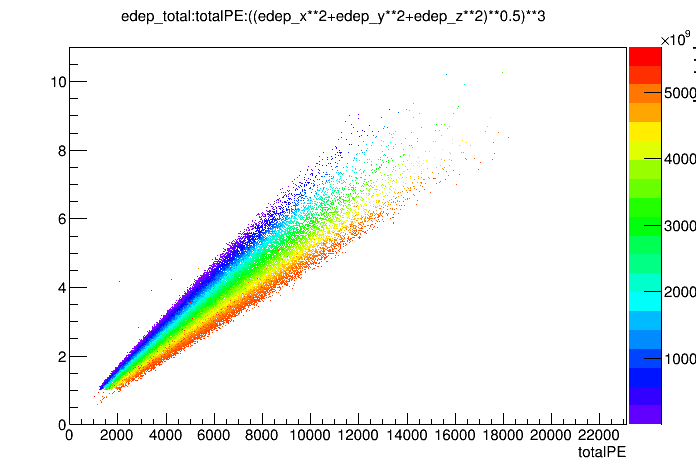
\includegraphics[width=6.5cm,keepaspectratio]{data/edep_total_vs_pe_vs_edepr3_small.png}
            \caption{不含本底的IBD事例}
        \end{figure}
        \column{6.5cm}
        \begin{figure}
            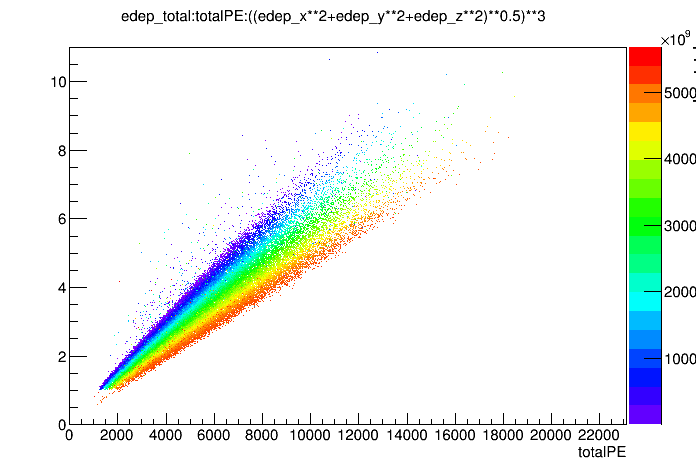
\includegraphics[width=6.5cm,keepaspectratio]{data/edep_total_vs_pe_vs_edepr3_mixed_small.png}
            \caption{含本底的IBD事例}
        \end{figure}
    \end{columns}
    含本底后,事例会变得异常。
\end{frame}

\begin{frame}
    \frametitle{一种检验信号是否含有本底的想法(cont.)}
    观察 $Edep(MeV) \over totalPE$ 与 $EdepR^{3}$ 的关系。
    由于Edep会比较小,如果在分母,结果会变得较大。因此,使用totalPE做分母。
    \begin{figure}
        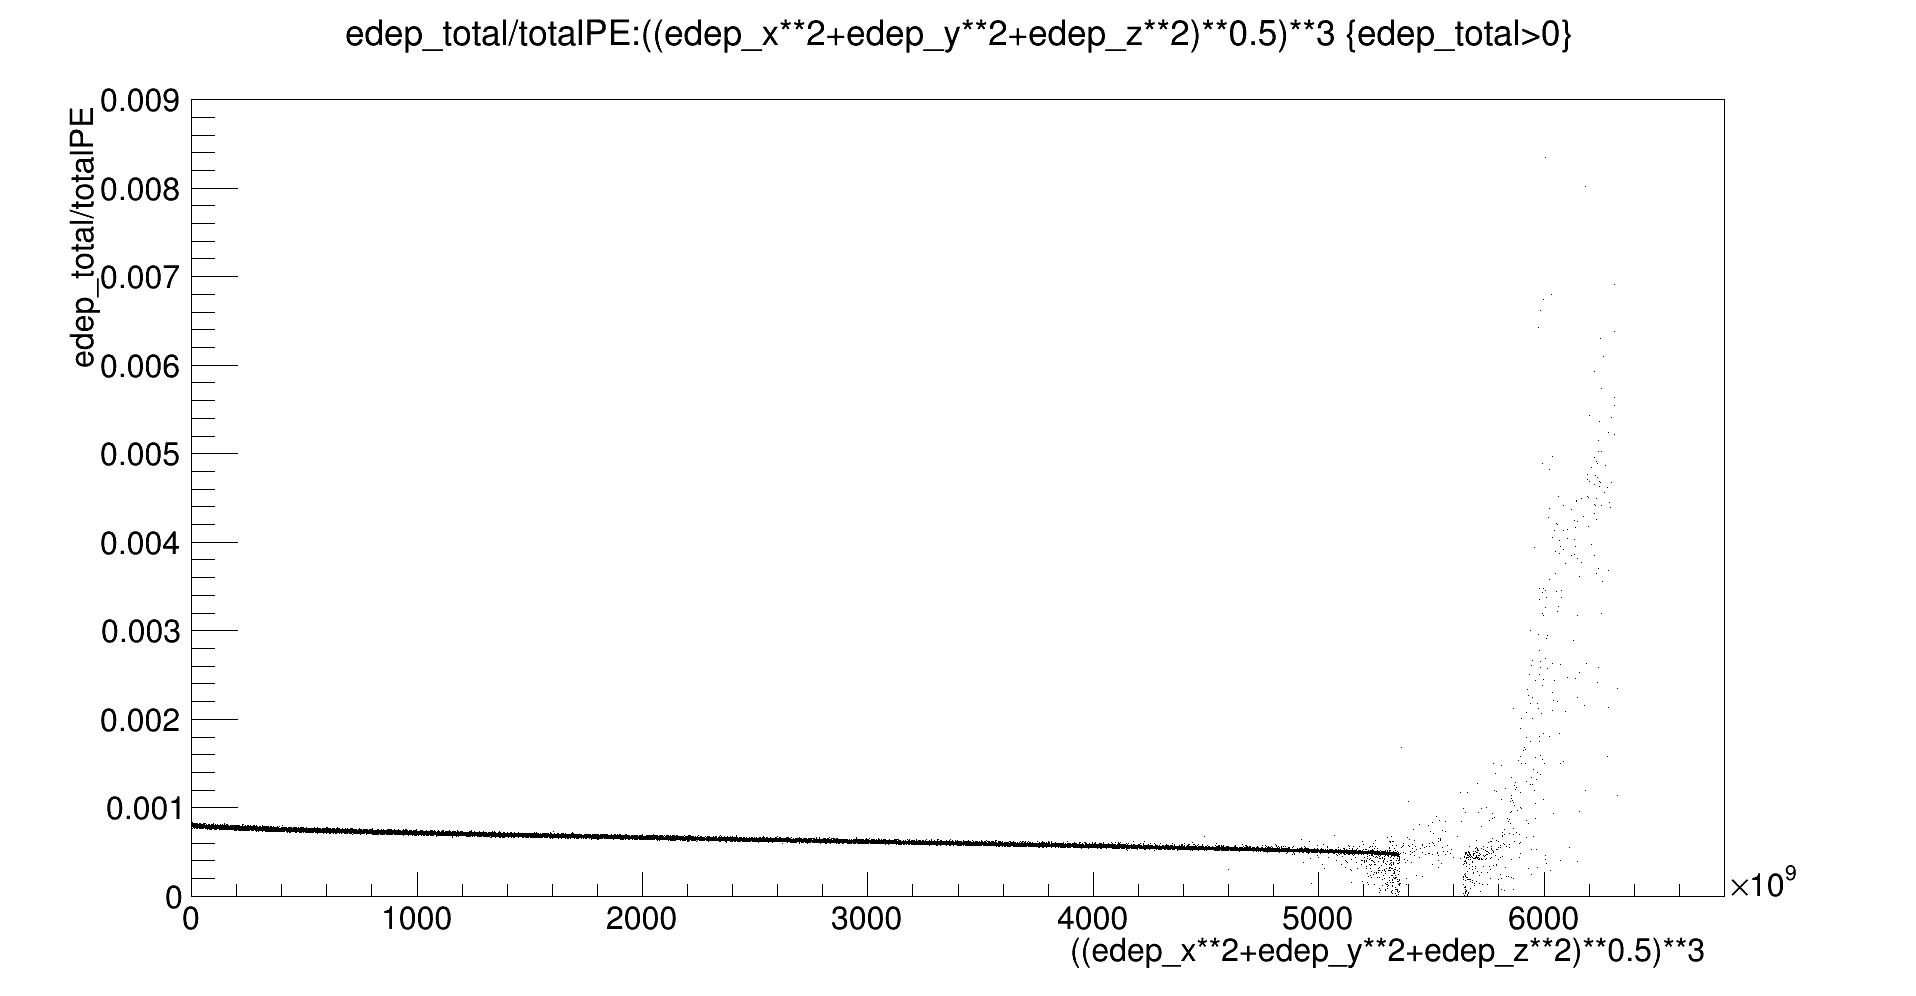
\includegraphics[width=11cm,keepaspectratio]{data/edep_total_div_totalPE_vs_edepr3.png}
        \caption{6130 MeV gamma 在30cm厚的有机玻璃罐方案下的结果}
    \end{figure}
\end{frame}

\begin{frame}
    \frametitle{液闪+有机玻璃+水屏蔽方案}
    这个方案液闪的半径仍为17.5m。有机玻璃罐厚度为10cm。
    此处主要研究本底的屏蔽情况。下面都是K40的情况。
    \begin{columns}
        \column{6.5cm}
        \begin{figure}
            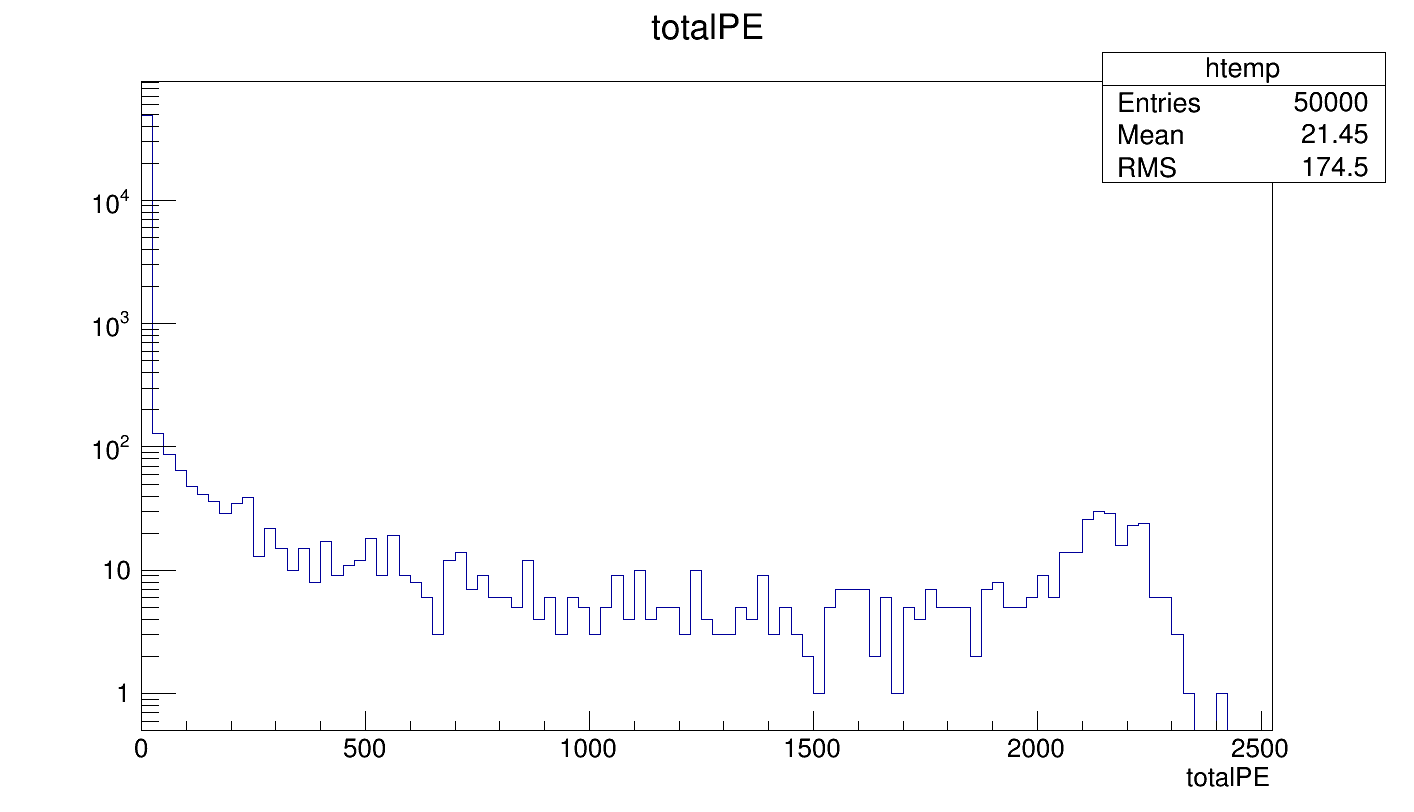
\includegraphics[width=6.5cm,keepaspectratio]{data/water_0.01m_K40_totalPE.png}
            \caption{PMT至有机玻璃1cm}
        \end{figure}
        \column{6.5cm}
        \begin{figure}
            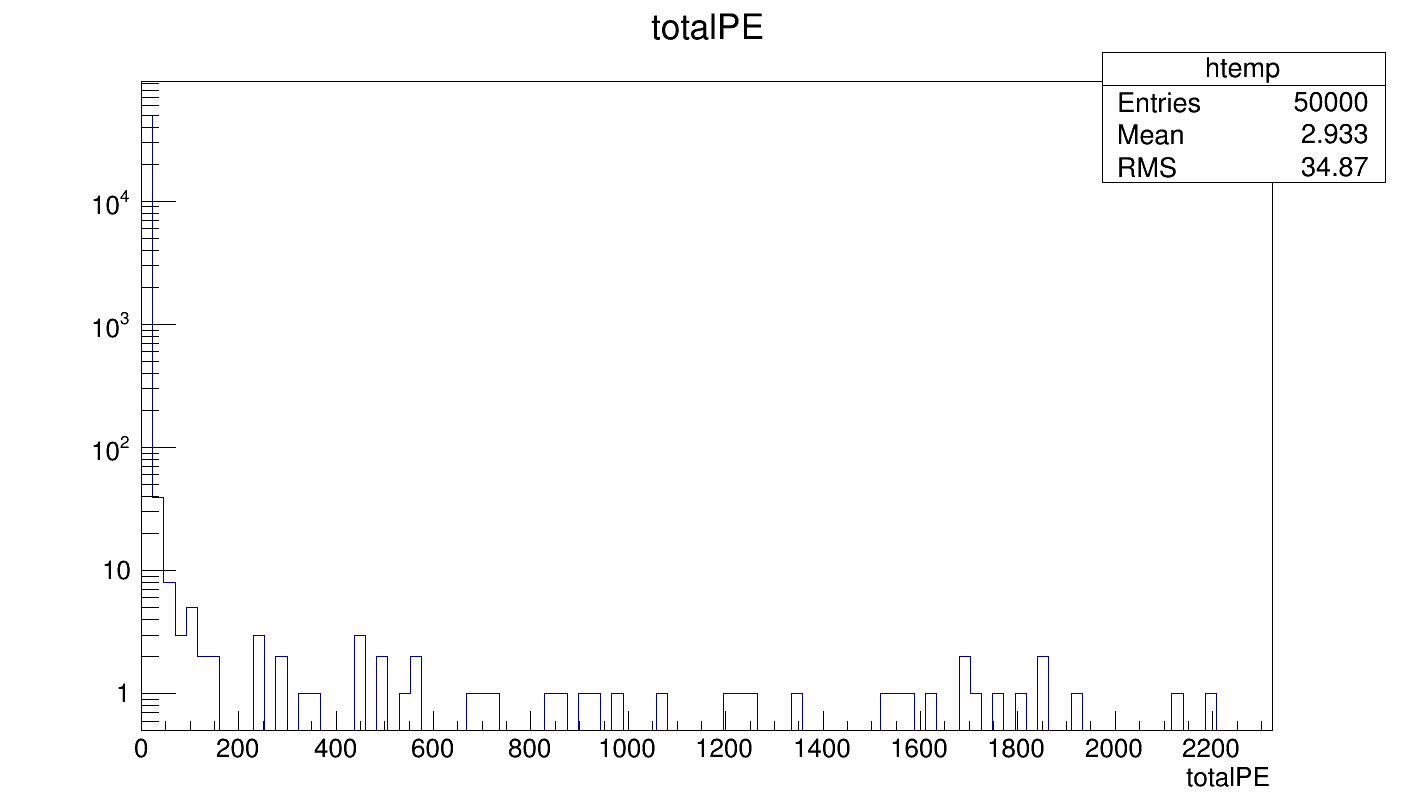
\includegraphics[width=6.5cm,keepaspectratio]{data/water_0.5m_K40_totalPE.png}
            \caption{PMT至有机玻璃0.5m}
        \end{figure}
    \end{columns}
\end{frame}

\begin{frame}
    \frametitle{液闪+有机玻璃+水屏蔽方案 (cont.)}
    \begin{columns}
        \column{6.5cm}
        \begin{figure}
            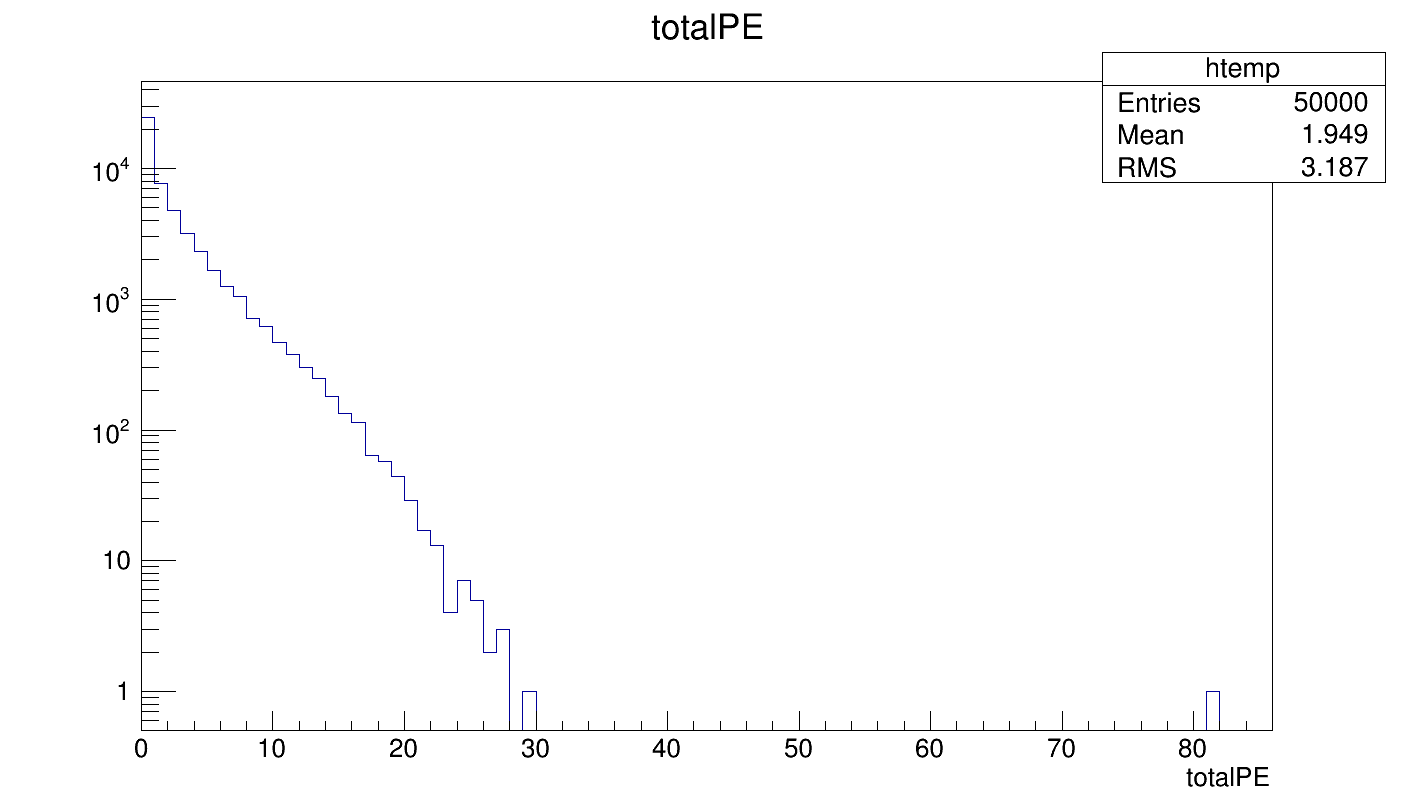
\includegraphics[width=6.5cm,keepaspectratio]{data/water_1.0m_K40_totalPE.png}
            \caption{PMT至有机玻璃1cm}
        \end{figure}
        \column{6.5cm}
        \begin{figure}
            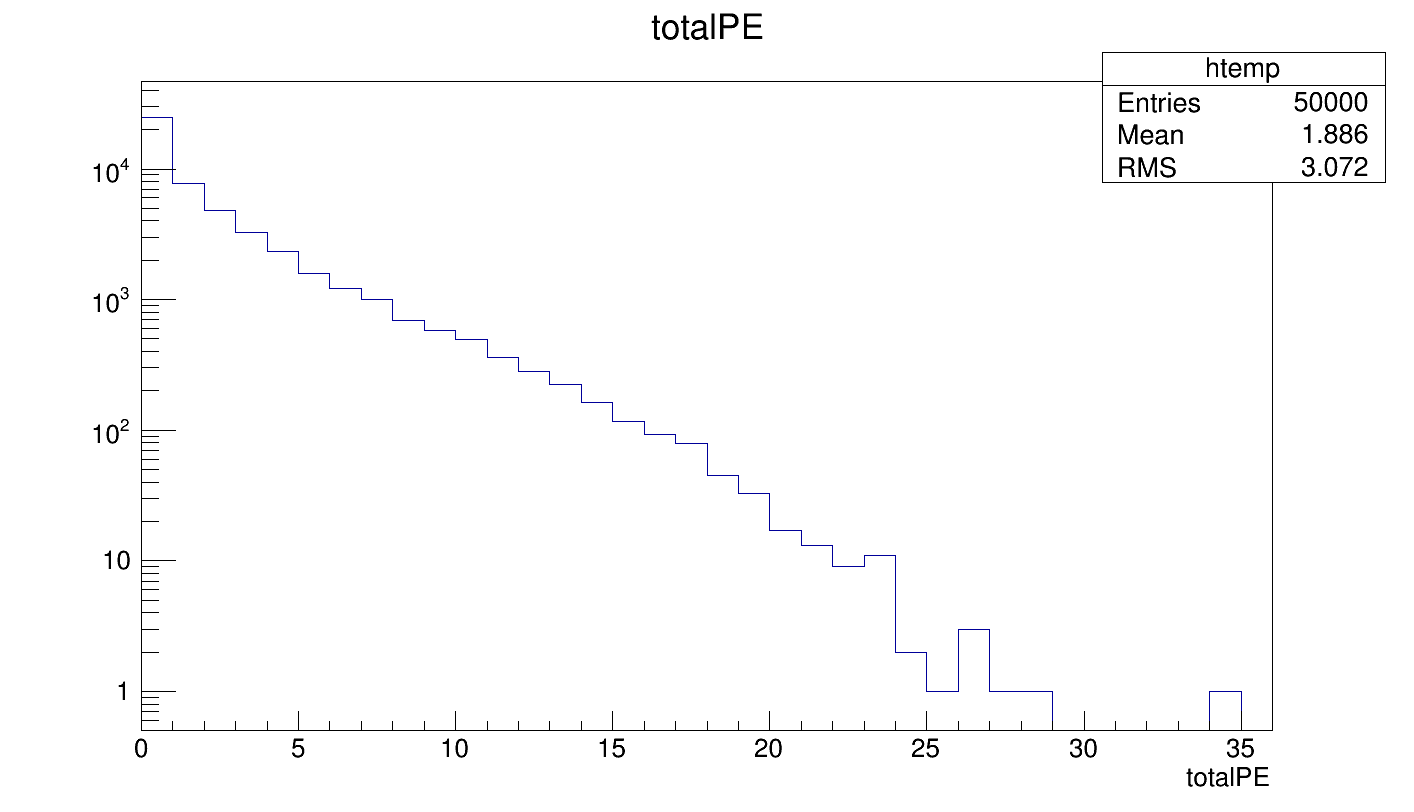
\includegraphics[width=6.5cm,keepaspectratio]{data/water_1.5m_K40_totalPE.png}
            \caption{PMT至有机玻璃0.5m}
        \end{figure}
    \end{columns}
\end{frame}

\begin{frame}
    \frametitle{有机玻璃罐方案}
    \begin{itemize}
        \item 此方案为有机玻璃罩方案的简化版。
        \item 目的在于研究PMT前方摆放{\em 一定厚度}的有机玻璃对本底的影响。
        \item 由于有机玻璃的存在,能量分辨率相对于纯钢罐有所变化。
        \item 随着有机玻璃罐厚度的增加,对于能量较高的6.13MeV
              的gamma在LS边缘部分可收集到更多的光子,因此分辨相对于
              纯钢罐方案变好。
        \item 而对于本底事例,由于在玻璃表面产生后,能立马在液闪中发光,
              因此,本底产生的影响仍然较大。
    \end{itemize}
\end{frame}

\begin{frame}
    \frametitle{不同有机玻璃罐厚度下的能量分辨率}
\begin{tabular}{|c|c|c|c|c|c|}
    \hline
    \multicolumn{6}{|c|}{无本底时的能量分辨率}
    \\
\hline
% line one
\multirow{2}{*}{\footnotesize 厚度}
 & \multirow{2}{*}{\footnotesize 2*0.511MeV}
 & \multirow{2}{*}{\footnotesize 2.22MeV}
 & {\footnotesize 1.173MeV,}
 & \multirow{2}{*}{\footnotesize 6.130MeV}
 & \multirow{2}{*}{$\sigma={{\mathnormal{p}_{0}}\over\sqrt{E}}$中的
                   $\mathnormal{p}_{0}$}
\\
& & & {\footnotesize 1.333MeV} & &
\\
\hline
% line two
10cm 
 & 0.029643
 & 0.023443
 & 0.021008
 & 0.015893
 & $0.0325\pm0.0017$
\\
% line three
15cm 
 & 0.029730
 & 0.023461
 & 0.020809
 & 0.015861
 & $0.0325\pm0.0016$
\\
% line four
20cm 
 & 0.029828
 & 0.023614
 & 0.020879
 & 0.015833
 & $0.0326\pm0.0016$
\\
% line five
25cm 
 & 0.029925
 & 0.023281
 & 0.021137
 & 0.015792
 & $0.0326\pm0.0016$
\\
% line six
30cm 
 & 0.029942
 & 0.023466
 & 0.020963
 & 0.015844
 & $0.0327\pm0.0016$
% end
\\
\hline
\end{tabular}

% TODO
\begin{tabular}{|c|c|c|c|c|c|}
    \hline
    \multicolumn{6}{|c|}{本底事例率1MHz时间窗口300ns时的能量分辨率}
    \\
\hline
% line one
\multirow{2}{*}{\footnotesize 厚度}
 & \multirow{2}{*}{\footnotesize 2*0.511MeV}
 & \multirow{2}{*}{\footnotesize 2.22MeV}
 & {\footnotesize 1.173MeV,}
 & \multirow{2}{*}{\footnotesize 6.130MeV}
 & \multirow{2}{*}{$\sigma={{\mathnormal{p}_{0}}\over\sqrt{E}}$中的
                   $\mathnormal{p}_{0}$}
\\
& & & {\footnotesize 1.333MeV} & &
\\
\hline
% line two
10cm 
 & 0.032655
 & 0.024767
 & 0.022166
 & 0.016552
 & $0.0350\pm0.0014$
\\
% line three
15cm 
 & 0.032815
 & 0.024923
 & 0.022043
 & 0.016577
 & $0.0351\pm0.0014$
\\
% line four
20cm 
 & 0.032856
 & 0.024968
 & 0.022118
 & 0.016448
 & $0.0351\pm0.0013$
\\
% line five
25cm 
 & 0.032745
 & 0.024908
 & 0.022436
 & 0.016406
 & $0.0351\pm0.0013$
\\
% line six
30cm 
 & 0.033812
 & 0.025007
 & 0.022318
 & 0.016615
 & $0.0357\pm0.0012$
% end
\\
\hline
\end{tabular}

\end{frame}

\begin{frame}
    \frametitle{有机玻璃罩方案}
    \begin{itemize}
        \item 为了更贴近真实的情况,我们初步研究了有机玻璃罩方案。
        \item 此处的有机玻璃罩主要是盖于PMT的顶部,未考虑封装PMT的尾部。
              \footnote{\footnotesize PMT尾部进行密封的方案可参考邓子艳,方肖,陈泉佑最近的工作。
                        他们考虑了在PMT表面存在液闪薄膜的情况。}
        \item 由于玻璃罩为圆柱体,有一定高度。并且考虑玻璃罩不能够重叠,使得PMT的覆盖率下降。
            \ref{pmt:lowcoverage}是有玻璃罩的。\ref{pmt:normcoverage}是纯钢罐方案的。
            \begin{equation} \label{pmt:lowcoverage}
                {N\pi{}r ^{2} \over 4\pi{}R^{2}} 
                = {13306 \cdot (255\mm)^{2} \over 4 \cdot (17.5\metre+20\cm)^{2}}
                = 69.04\%
            \end{equation}
            \begin{equation} \label{pmt:normcoverage}
                {N\pi{}r ^{2} \over 4\pi{}R^{2}} 
                = {14159 \cdot (255\mm)^{2} \over 4 \cdot (17.5\metre)^{2}}
                = 75.16\%
            \end{equation}
        \item 覆盖率的下降,导致收集的光子数下降,能量分辨率下降。
              
    \end{itemize}
\end{frame}

\begin{frame}
    \frametitle{有机玻璃罩示意图}
    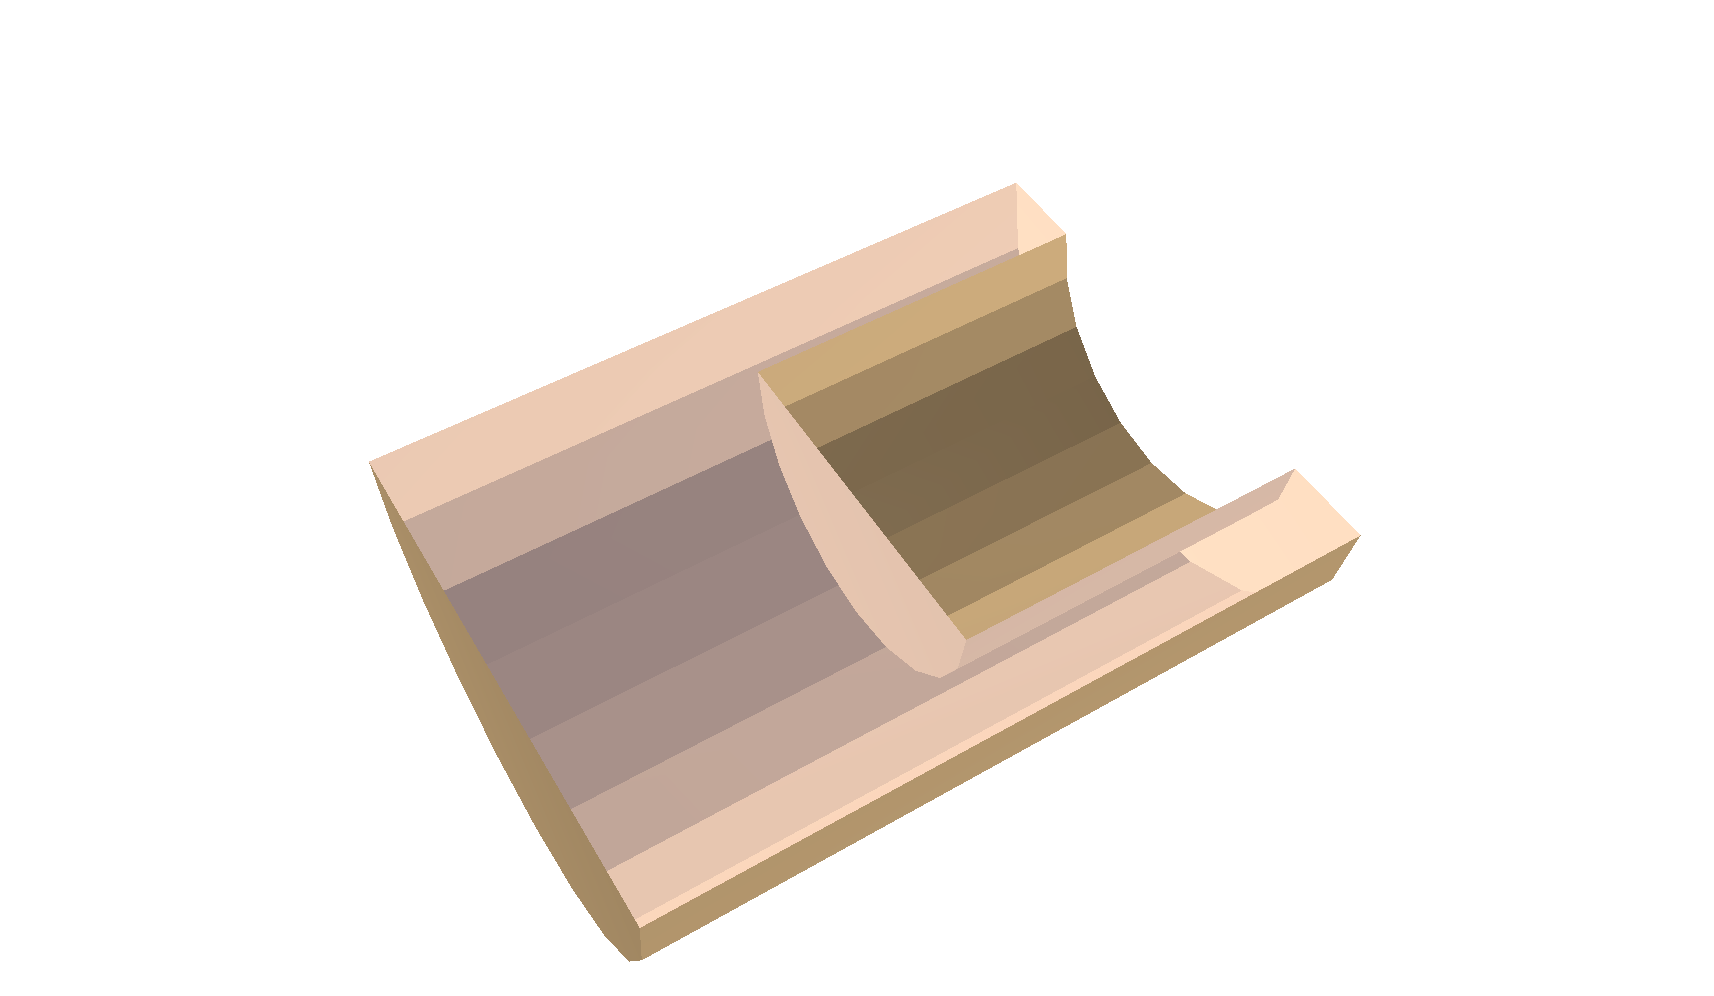
\includegraphics[width=12cm,keepaspectratio]{data/PMT_HAT.png}
\end{frame}

\begin{frame}
    \frametitle{1mm液闪对本底的影响}
    \begin{itemize}
        \item 探测器构造为
            \begin{itemize}
                \item 基于纯钢罐方案。
                \item 中心为半径为1mm的球,材料为发光的液闪。
                \item 其他部分的液闪设置为不发光。
            \end{itemize}
        \item 对于U, Th, K, 需要考虑$\alpha$, $\beta$, $\gamma$放射性。
        \item 对于$\alpha$粒子,需要考虑淬灭效应。
        \item $\alpha$粒子在$1\mm$液闪中大部分能够沉积。
        \item $\gamma$则沉积得较少。
        \item $\beta$则介于两者之间。
        \item 尽管只有$1\mm$的厚度,PMT上仍然能够产生1K多的光电子。
        \item 这些粒子如果从PMT玻璃飞出,到液闪后将会放出大量的光子。
              因此我们需要对本底进行有效的屏蔽。
        \item 如果在考虑时间窗口,那么会引入更多的光电子。
    \end{itemize}
\end{frame}

\begin{frame}
    \frametitle{对于Th,$\alpha$粒子动能,沉积能量及光电子的关系}
    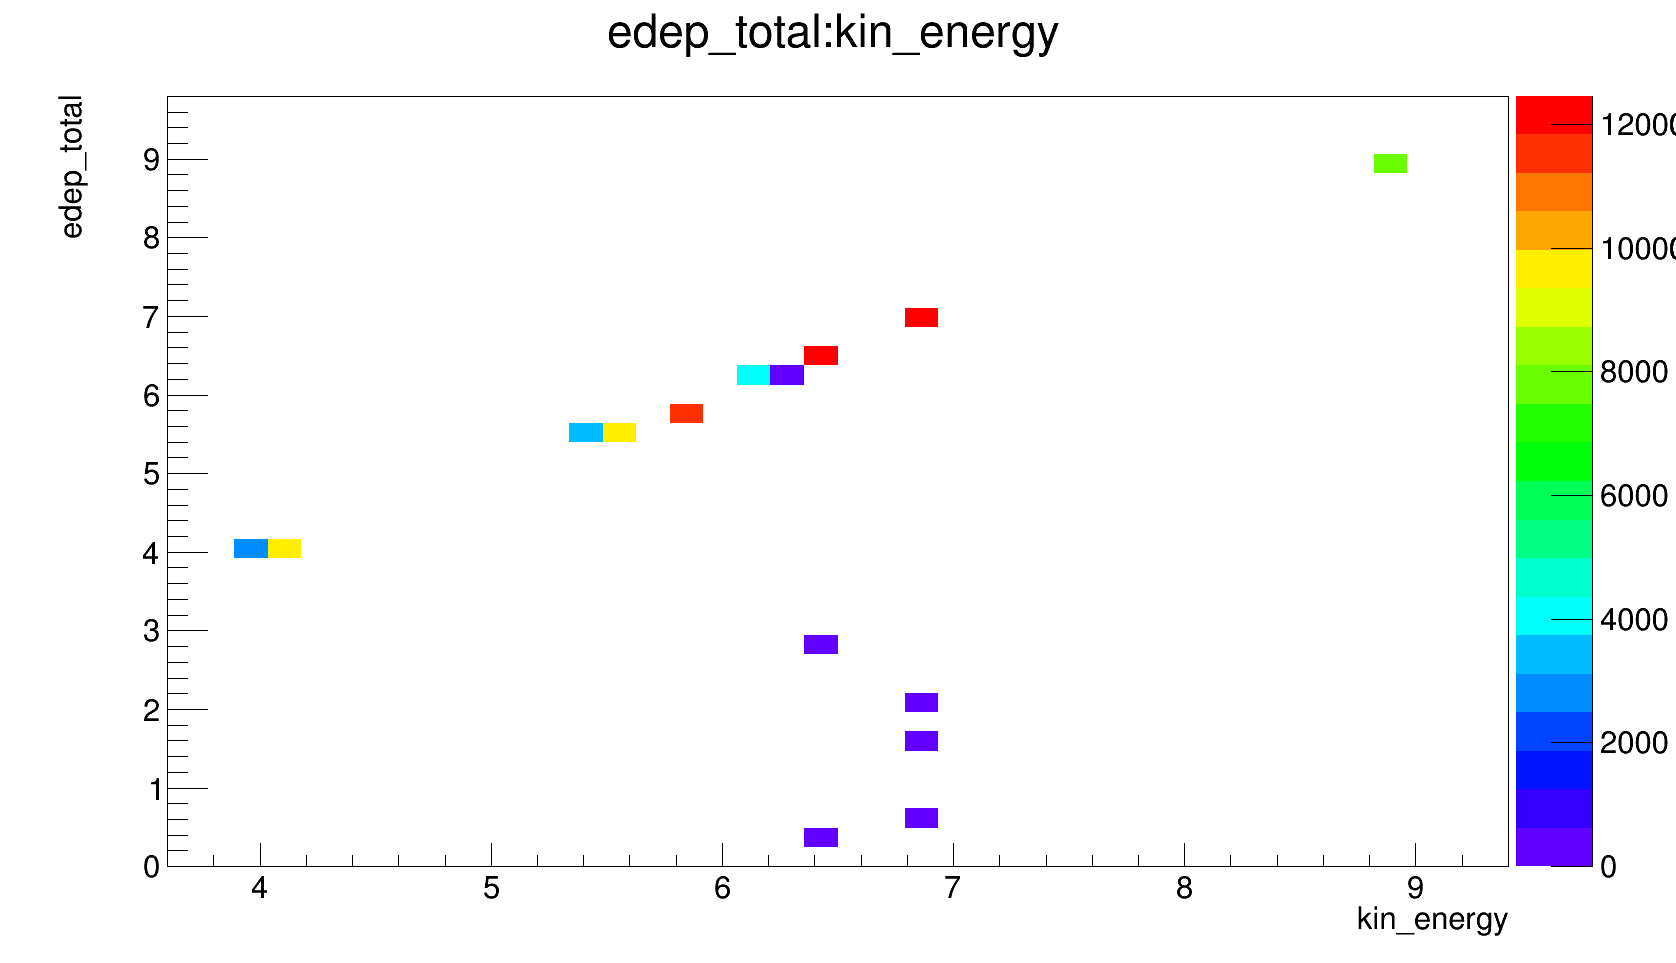
\includegraphics[width=12cm,height=4cm]{data/Th_alpha_edep_vs_kine.png}

    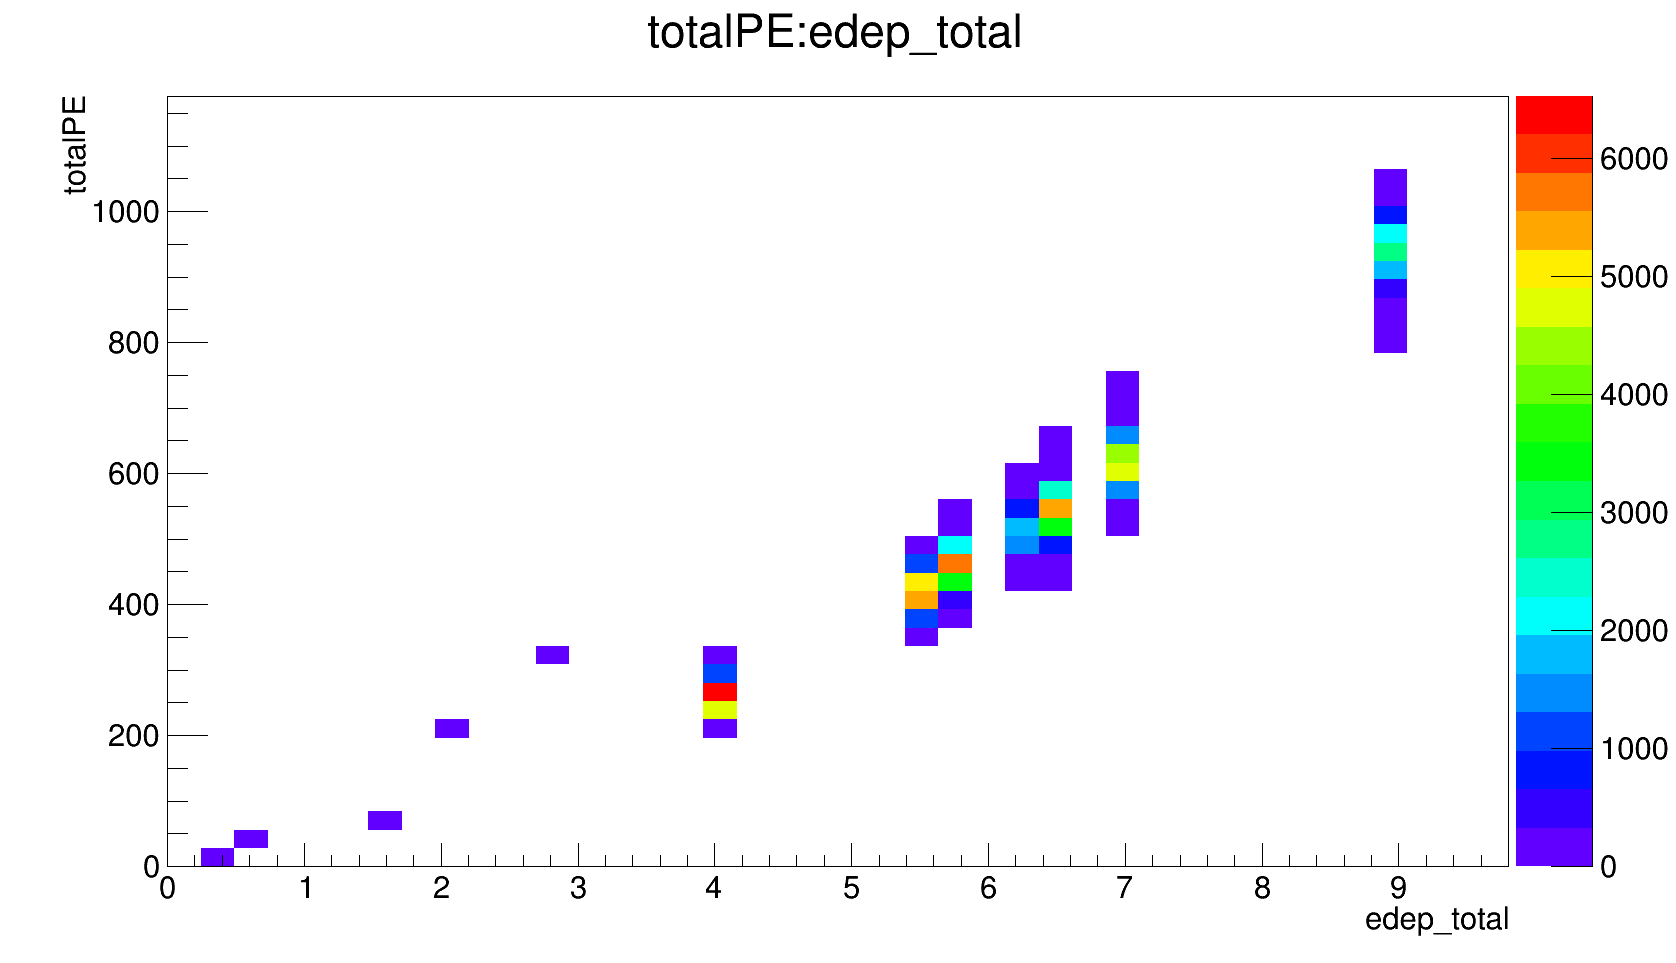
\includegraphics[width=12cm,height=4cm]{data/Th_alpha_totalPE_vs_edep.png}
\end{frame}

\begin{frame}
    \frametitle{对于U,$\alpha$粒子动能,沉积能量及光电子的关系}
    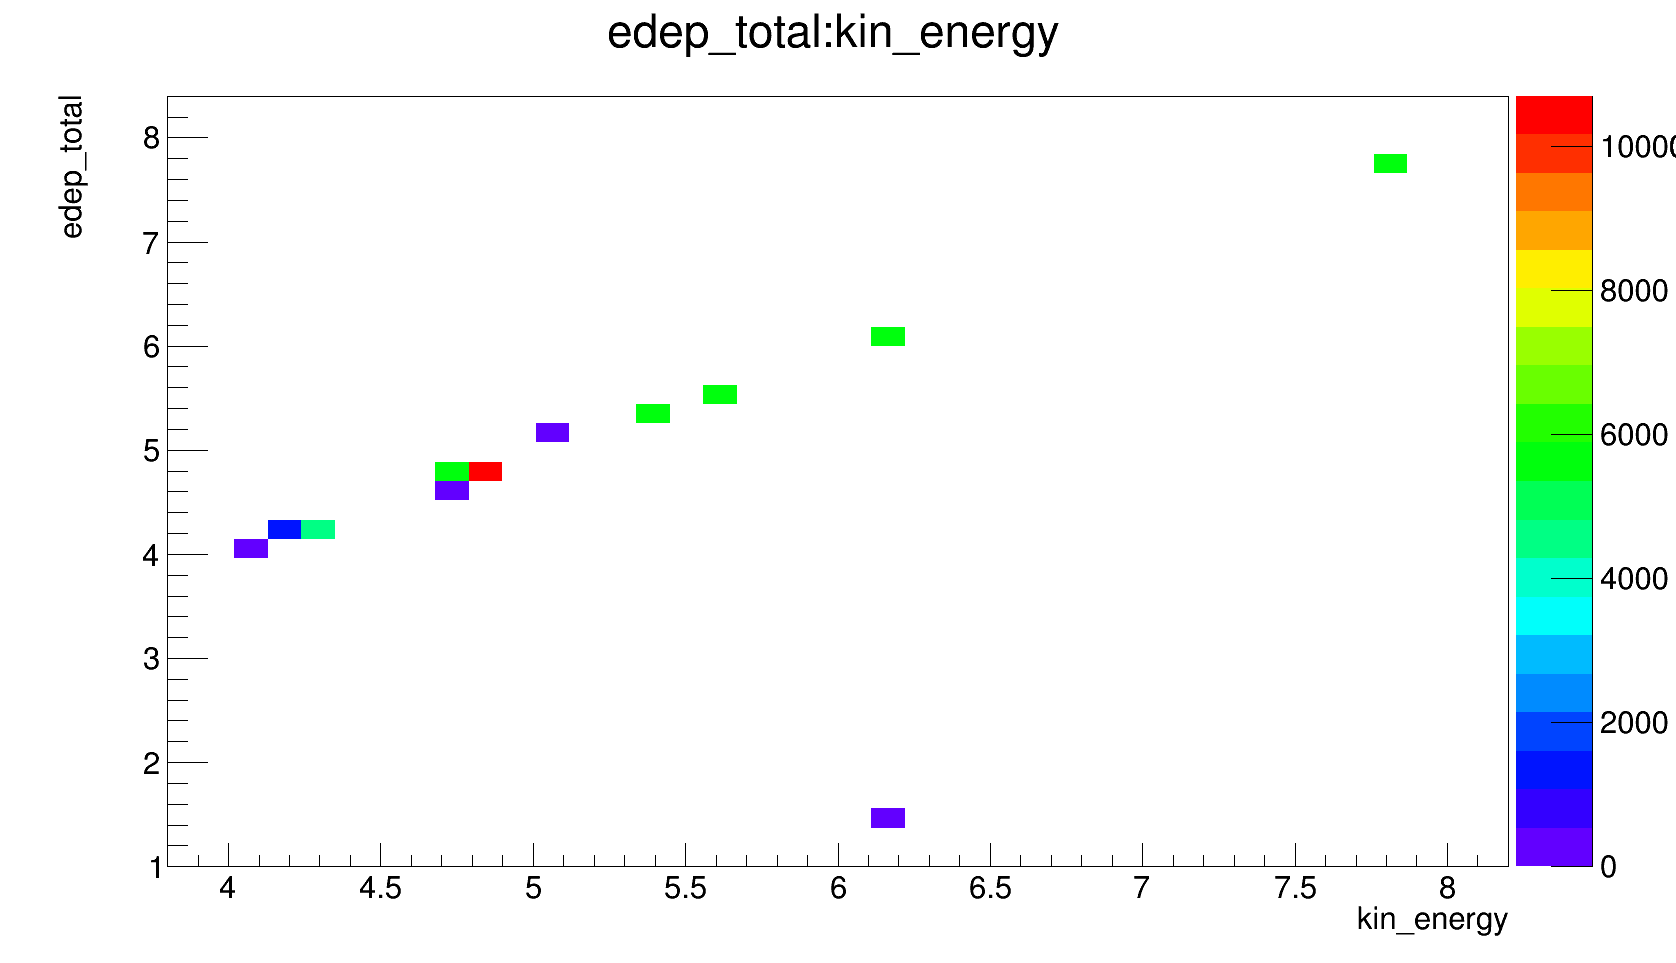
\includegraphics[width=12cm,height=4cm]{data/U_alpha_edep_vs_kine.png}

    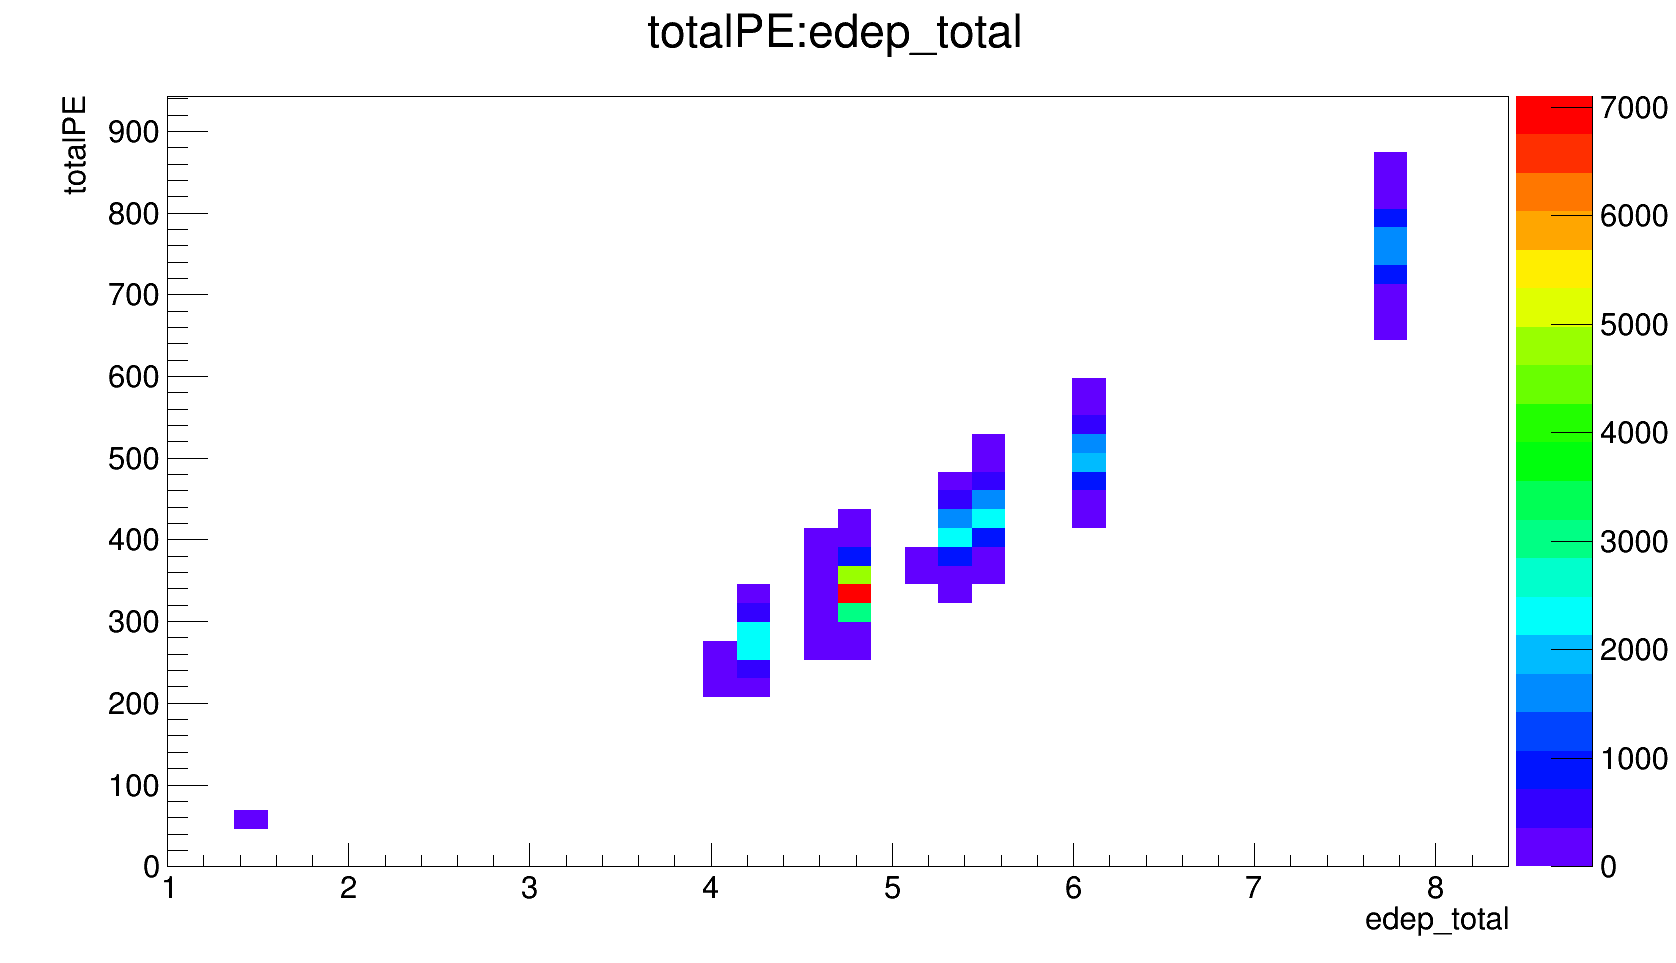
\includegraphics[width=12cm,height=4cm]{data/U_alpha_totalPE_vs_edep.png}
\end{frame}

\begin{frame}
    \frametitle{对于Th,$\beta$粒子动能,沉积能量及光电子的关系}
    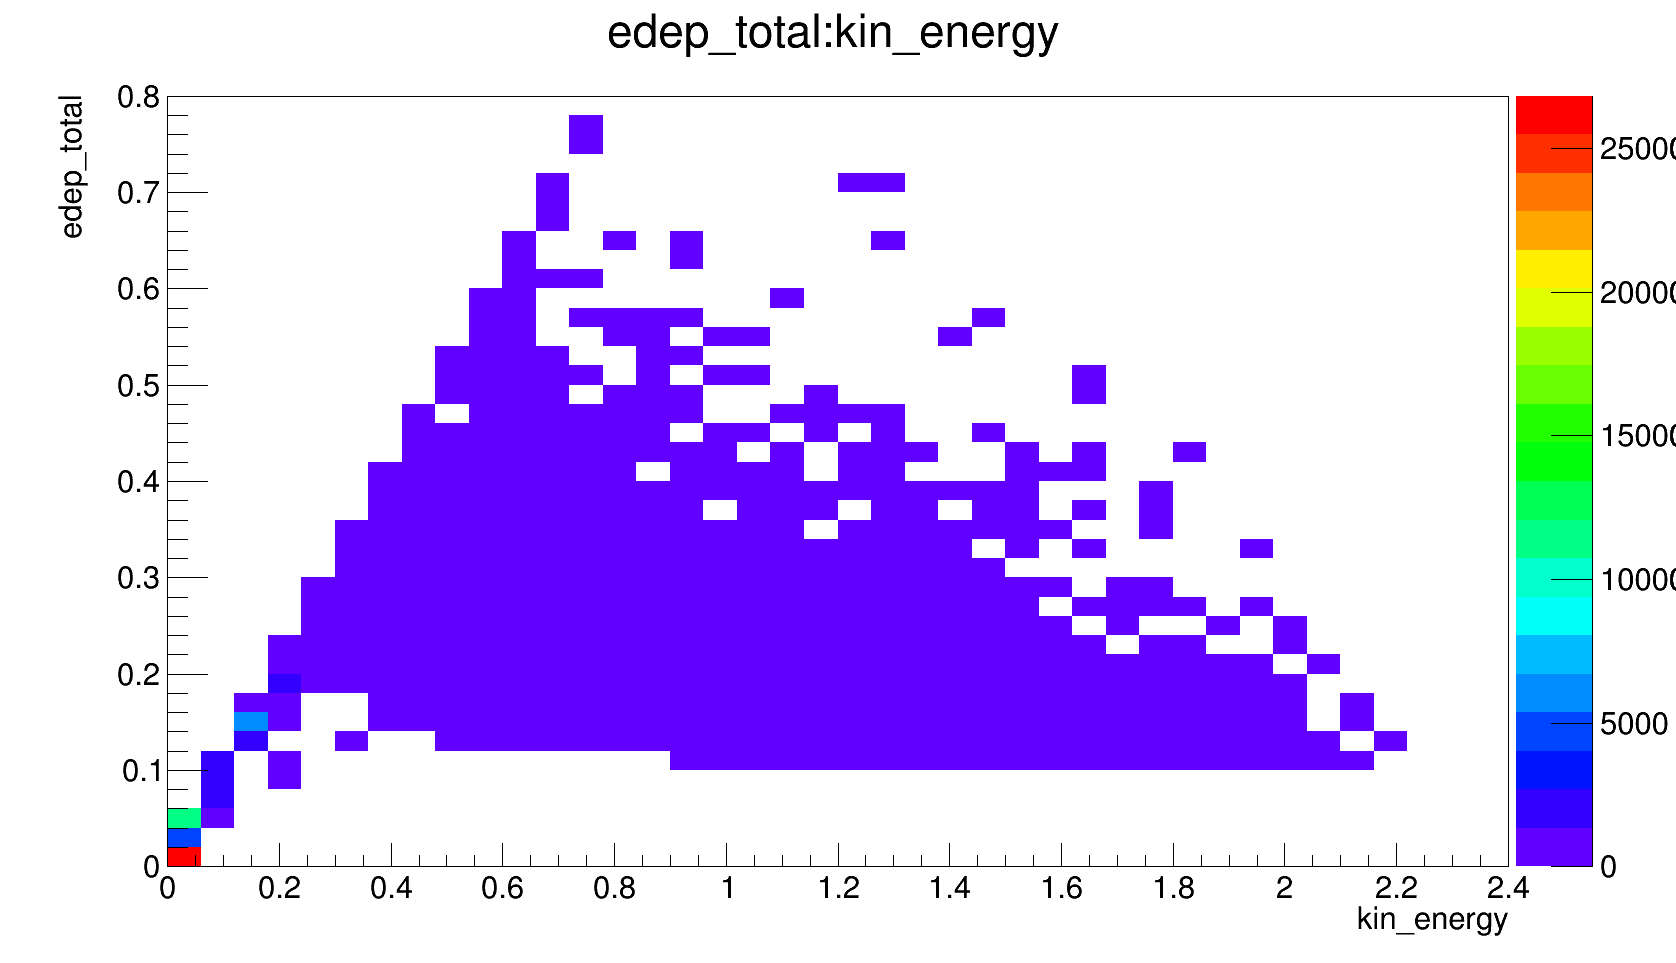
\includegraphics[width=12cm,height=4cm]{data/Th_beta_edep_vs_kine.png}

    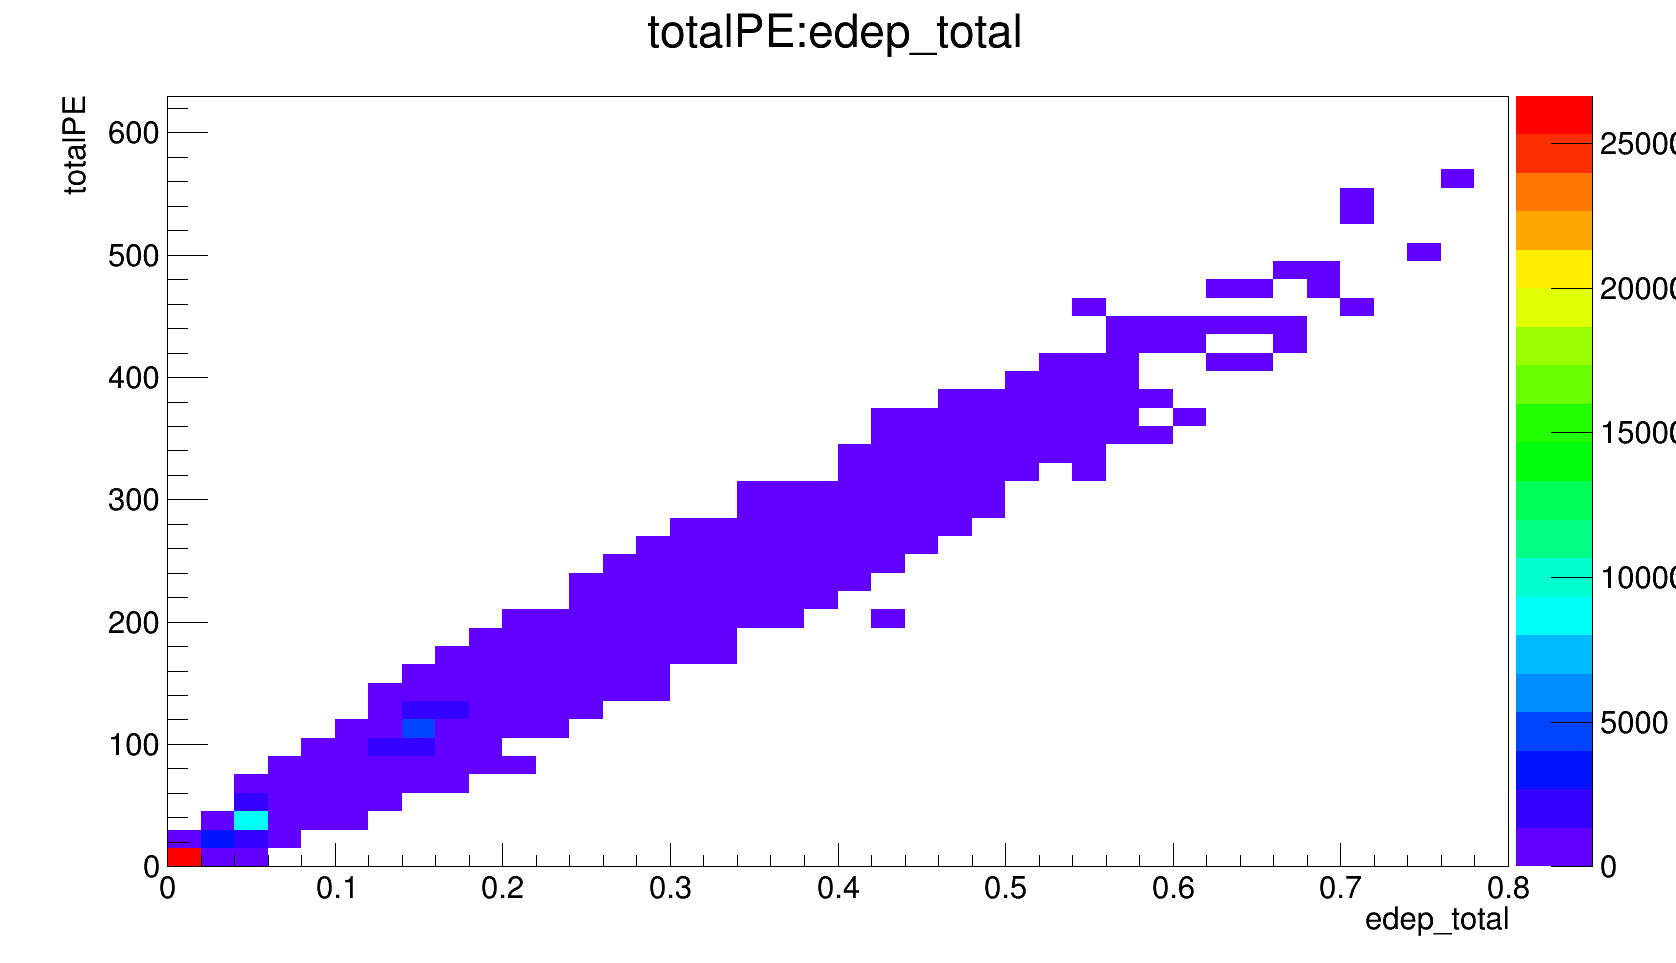
\includegraphics[width=12cm,height=4cm]{data/Th_beta_totalPE_vs_edep.png}
\end{frame}

\begin{frame}
    \frametitle{对于U,$\beta$粒子动能,沉积能量及光电子的关系}
    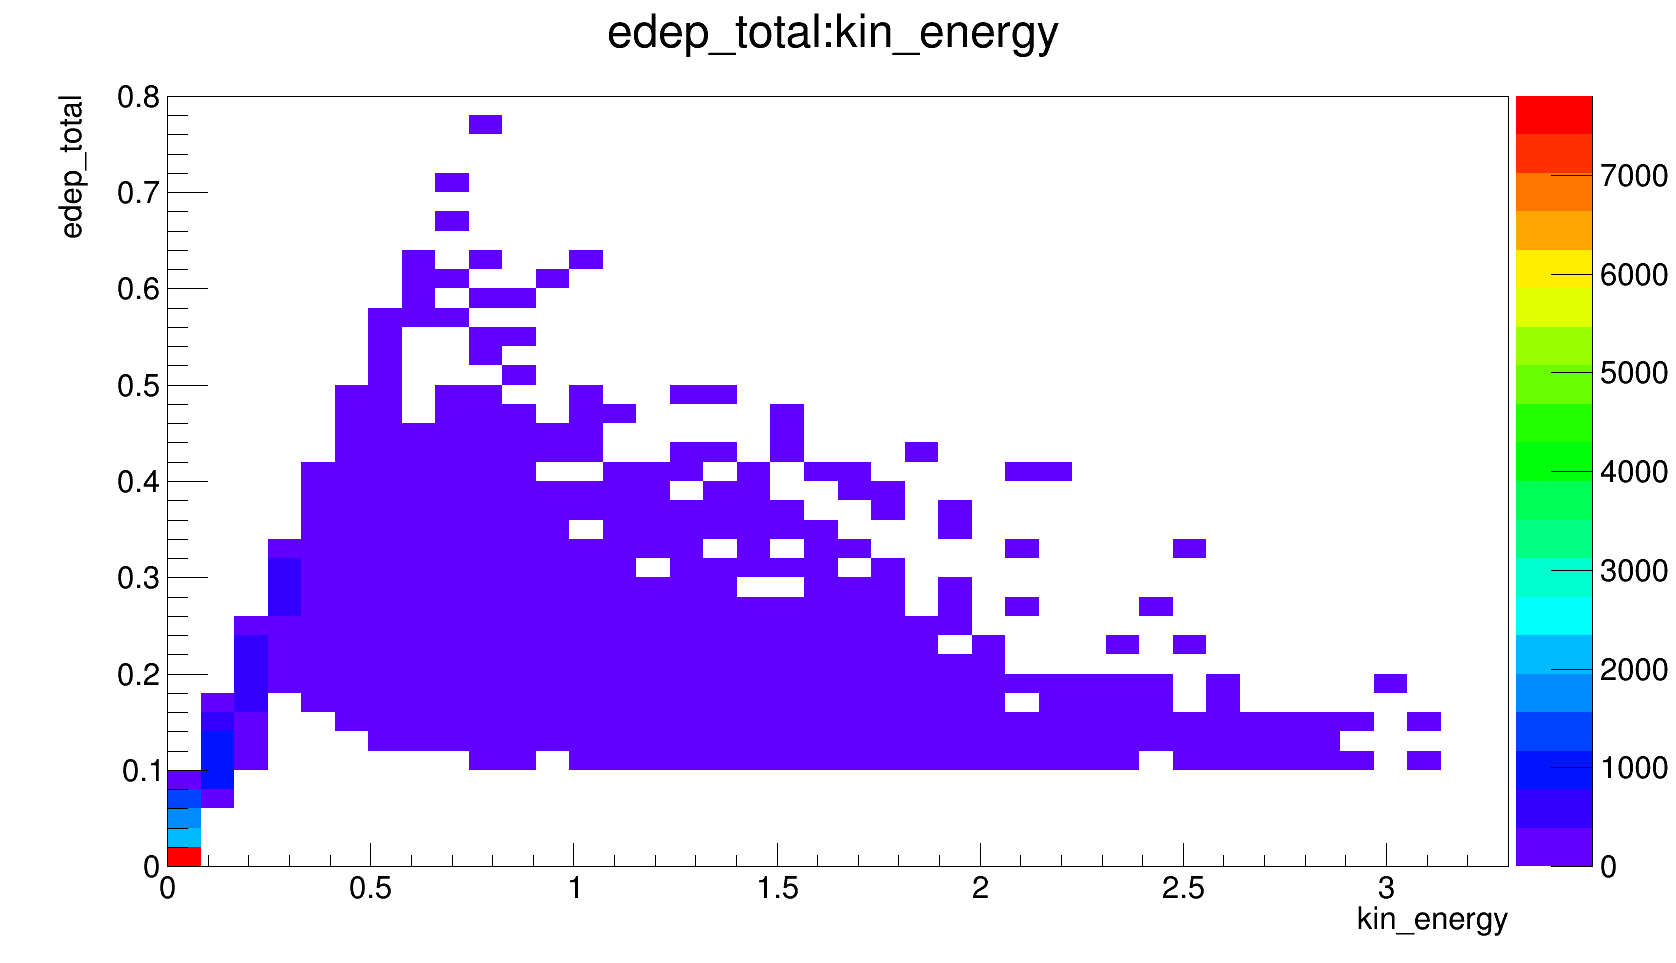
\includegraphics[width=12cm,height=4cm]{data/U_beta_edep_vs_kine.png}

    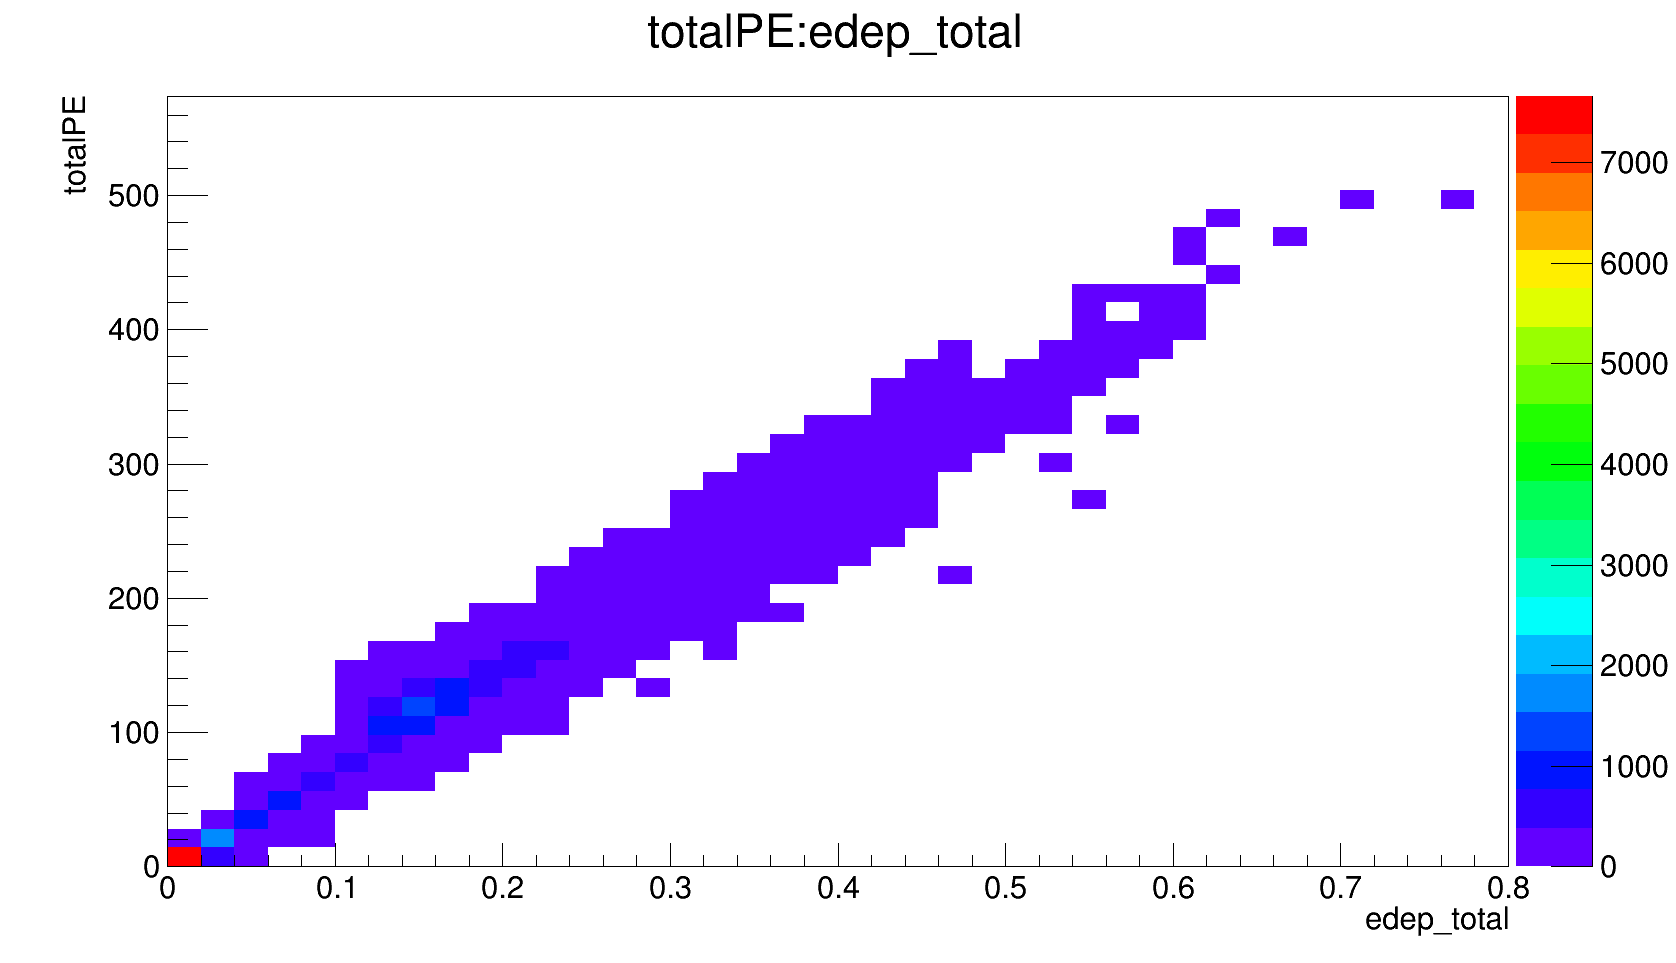
\includegraphics[width=12cm,height=4cm]{data/U_beta_totalPE_vs_edep.png}
\end{frame}

\begin{frame}
    \frametitle{对于Th,$\gamma$粒子动能,沉积能量及光电子的关系}
    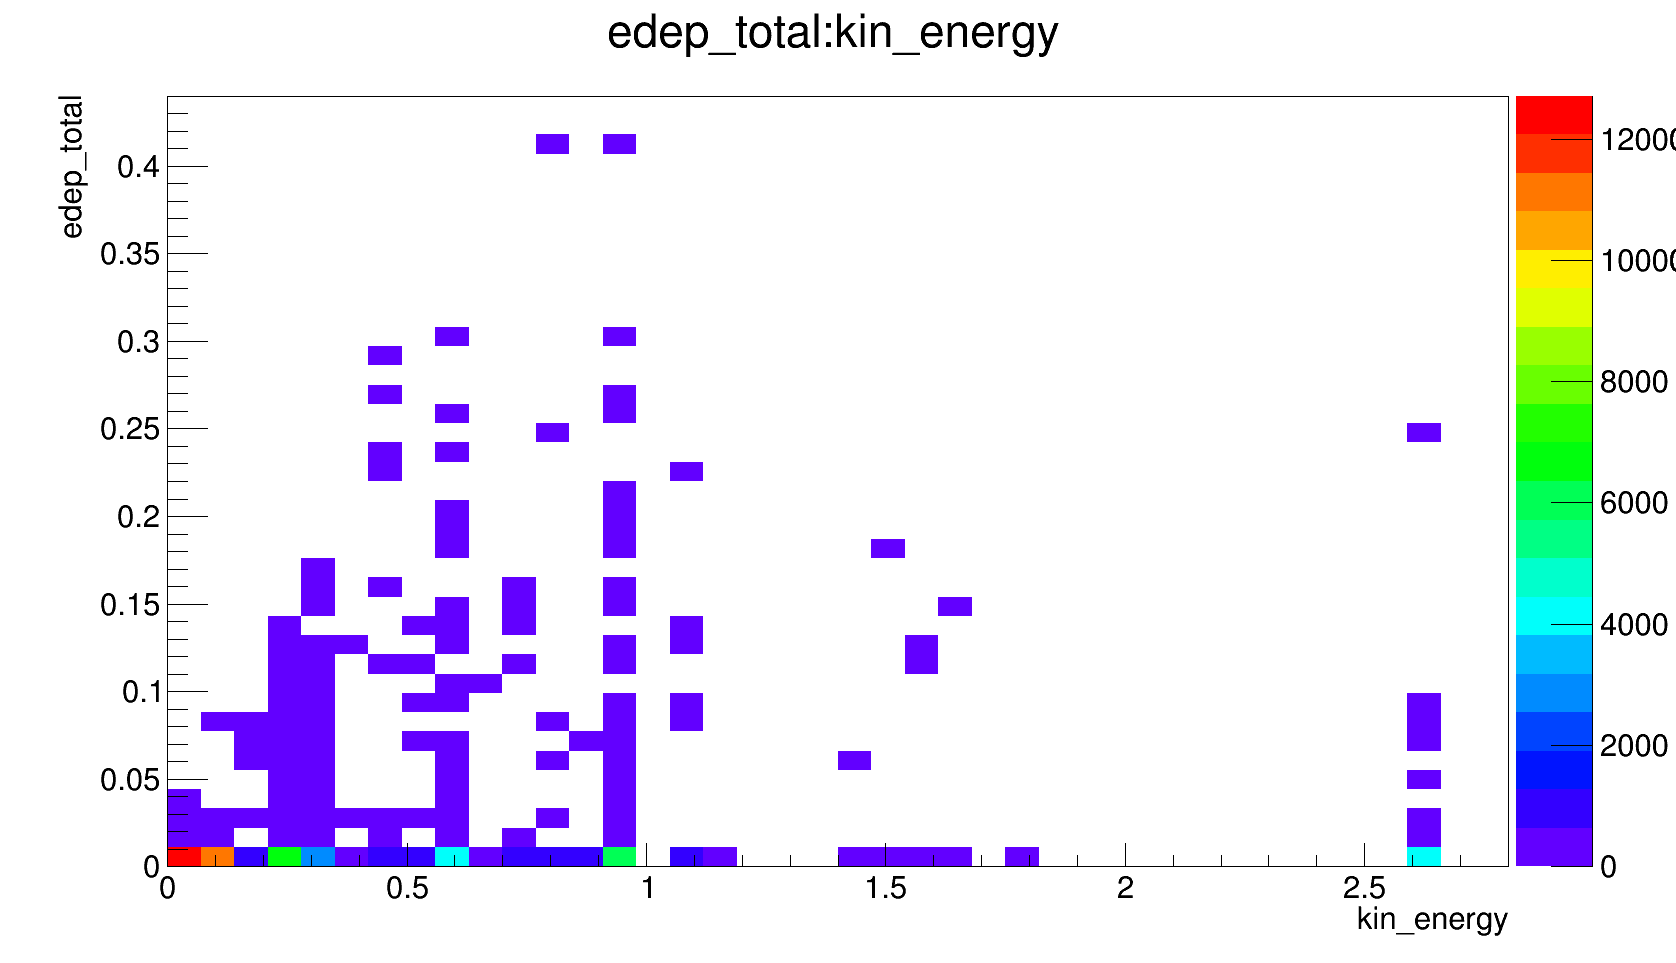
\includegraphics[width=12cm,height=4cm]{data/Th_gamma_edep_vs_kine.png}

    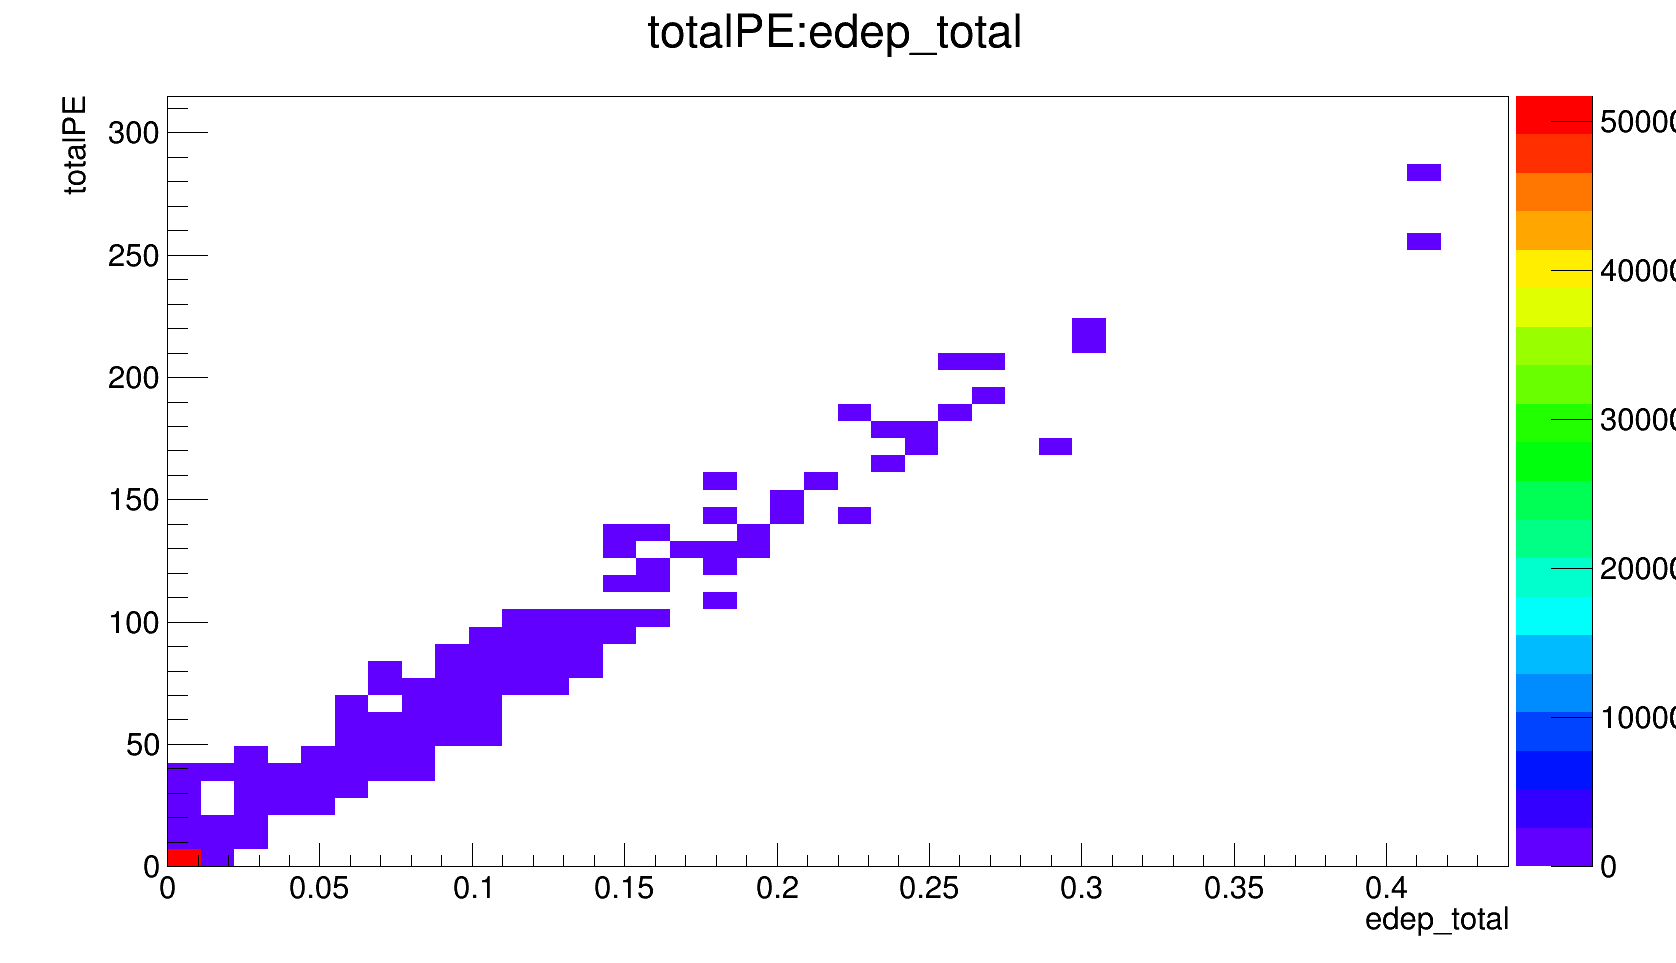
\includegraphics[width=12cm,height=4cm]{data/Th_gamma_totalPE_vs_edep.png}
\end{frame}

\begin{frame}
    \frametitle{对于U,$\gamma$粒子动能,沉积能量及光电子的关系}
    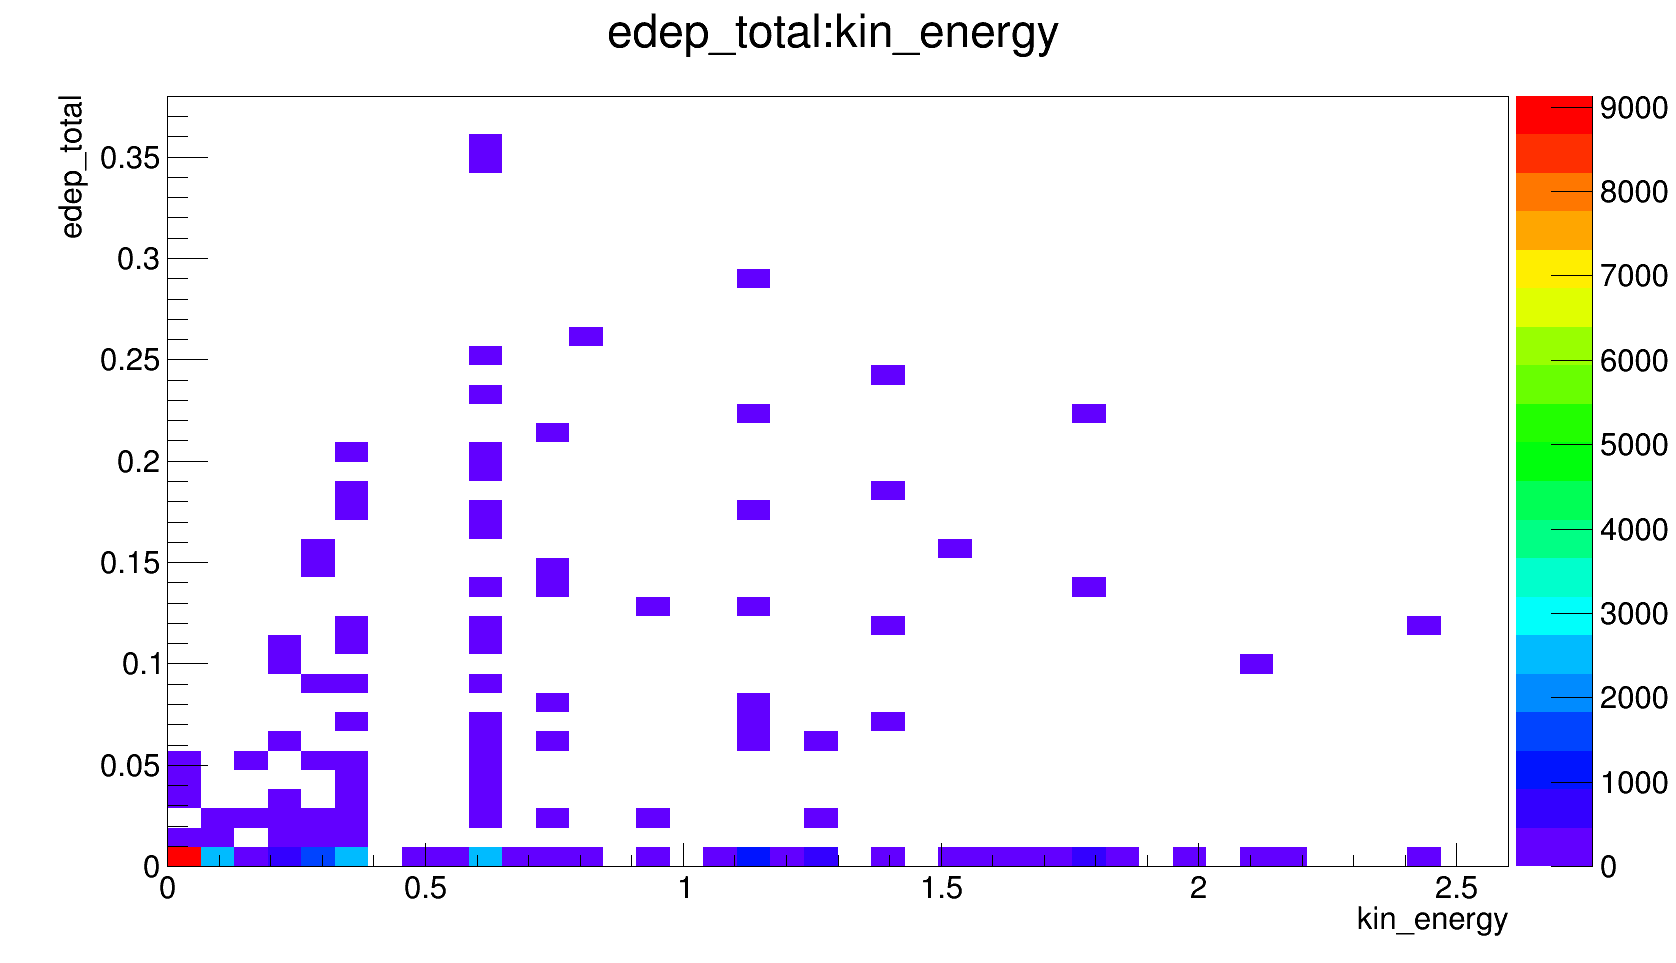
\includegraphics[width=12cm,height=4cm]{data/U_gamma_edep_vs_kine.png}

    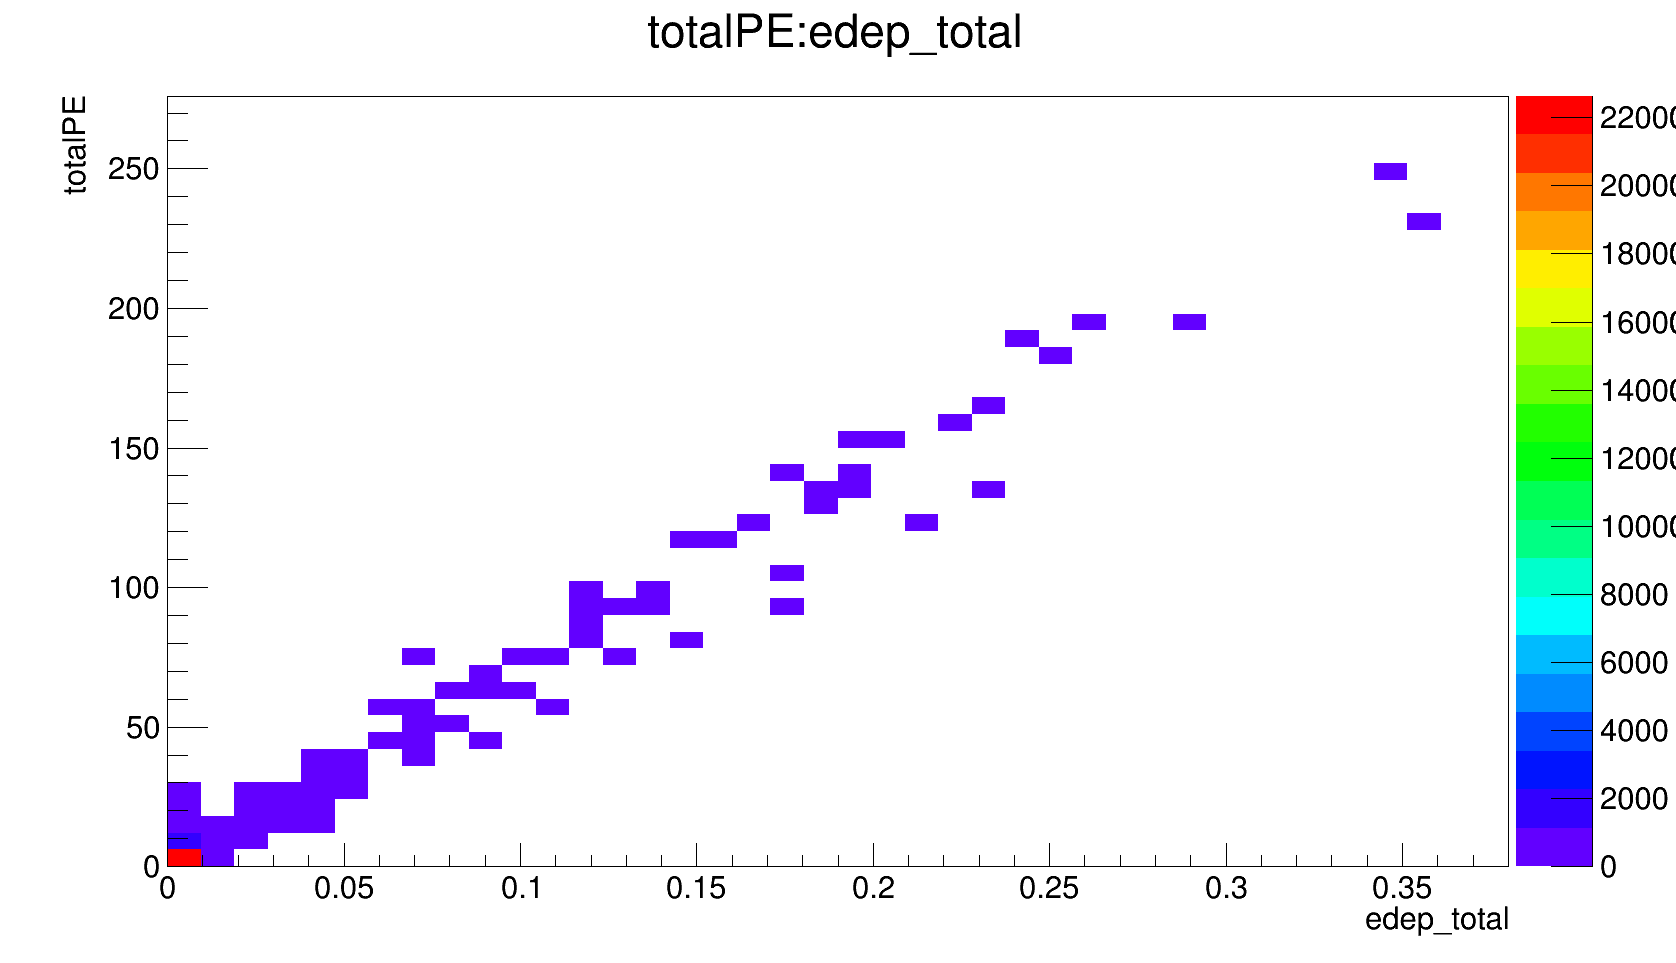
\includegraphics[width=12cm,height=4cm]{data/U_gamma_totalPE_vs_edep.png}
\end{frame}

\subsection{基于Sniper的模拟程序}

\newsavebox{\NoviceJobOptions}
\begin{lrbox}{\NoviceJobOptions}
\begin{lstlisting}[language=c++]
#include "$DETSIMROOT/share/jobOptions.txt"
Sniper.Dlls += {"Novice01"};
SvcMgr.Contents += {"ExN01Factory"};

Sniper.Cycler = "NormCycler";
Sniper.InputSvc = "NONE";

DetSim.DetFactory = "ExN01Factory";
DetSim.RunMac = "run.mac";

Sniper.EvtMax   = 2;
Sniper.LogLevel = 3; // INFO
\end{lstlisting}
\end{lrbox}


\begin{frame}
    \frametitle{基于Sniper离线框架的模拟}
    \begin{itemize}
        \item Sniper是新的软件框架,追求简洁,适合非对撞实验。
        \item 主要提供了算法,服务和工具。
        \item 参考邓子艳老师的工作,对Geant4中{\tt RunManager}进行了改造。
              使其更适合于Sniper这个框架。
        \item 为了使原有的geant4程序修改最小,需要额外提供一个抽象工厂,
              这样基于Sniper的DetSim会根据此工厂自动构建探测器。
    \end{itemize}
    \par\usebox{\NoviceJobOptions}
\end{frame}

\newsavebox{\NoviceHeader}
\begin{lrbox}{\NoviceHeader}
\begin{lstlisting}[language=c++]
class ExN01Factory:  virtual public SvcBase , 
                     virtual public IDetSimFactory {
public:
    ExN01Factory(const std::string& name);
    virtual ~ExN01Factory();

    virtual G4VUserDetectorConstruction* createDetectorConstruction();
    virtual G4VUserPhysicsList* createPhysicsList();
    virtual G4VUserPrimaryGeneratorAction* createPrimaryGenerator();

    virtual bool initialize();
    virtual bool finalize();
};
\end{lstlisting}
\end{lrbox}

\begin{frame}
    \frametitle{Novice 01 需要提供的抽象工厂:头文件}
    \par\usebox{\NoviceHeader}
\end{frame}

\newsavebox{\NoviceImpl}
\begin{lrbox}{\NoviceImpl}
\begin{lstlisting}
G4VUserDetectorConstruction*
ExN01Factory::createDetectorConstruction()
{   
    return new ExN01DetectorConstruction;
}

G4VUserPhysicsList*
ExN01Factory::createPhysicsList()
{   
    return new ExN01PhysicsList;
}

G4VUserPrimaryGeneratorAction*
ExN01Factory::createPrimaryGenerator()
{   
    return new ExN01PrimaryGeneratorAction;
}
\end{lstlisting}
\end{lrbox}

\begin{frame}
    \frametitle{Novice 01 需要提供的抽象工厂:实现}
    \par\usebox{\NoviceImpl}
\end{frame}


\section{BESDIRAC传输系统}
    \begin{frame}
    \begin{center}
        \LARGE BESDIRAC及传输系统
    \end{center}
\end{frame}

\begin{frame}
    \frametitle{BESDIRAC及传输系统}
    \begin{itemize}
        \item 为了在网格站点中都能够使用BESDIRAC中的程序,
              我们开始发布BESDIRAC。
        \item 研究学习网页前端库ExtJS2。
        \item 开发了数据传输系统的Web Portal。
        \item 程序组成
            \begin{itemize}
                \item 
            \end{itemize}
    \end{itemize}
\end{frame}

\section{小结}
    \begin{frame}
    \begin{center}
        \LARGE 小结
    \end{center}
\end{frame}

\begin{frame}
    \frametitle{小结}
    \begin{itemize}
        \item 此阶段中,我们对PMT的构造进行重构,
              以适应有机玻璃罩及模块的情形。
              并使得PMT的位置坐标可以从文件读取(由硬件组提供坐标)。
              PMTManager的设计已被纯钢罐方案和模块方案采用。
              在产生子方面,目前支持在特定Volume中产生粒子。
              支持全局/局部的变换。
        \item 在Sniper框架方面,Sniper已经支持Python。
              期间主要研究了几种实现。
              目前已经使用C++模板元编程技术实现了Sniper Python的脚本配置。
        \item 网格计算方面,开始发布了BESDIRAC。
              除了继续完善数据传输系统,还学习编写了相应的Web Portal。
    \end{itemize}
\end{frame}


\section*{end}
\begin{frame}
    \begin{center}
        \LARGE Q \& A
    \end{center}
\end{frame}

\end{document}
